\documentclass[10pt,a4paper]{article}
\usepackage[utf8]{inputenc}
\usepackage[english]{babel}
\usepackage{amsmath}
\usepackage{amsthm}
\usepackage{amsfonts}
\usepackage{amssymb}
\usepackage{graphicx}
\usepackage[font=small]{caption}
\usepackage{wrapfig}
\usepackage{subfig}
\usepackage[a4paper,width=140mm,top=25mm,bottom=25mm]{geometry}
\author{Philipp Weder}
\title{\textbf{Final Report - Research Internship}}
\date{}





% packages for layout
\usepackage{fancyhdr}
\pagestyle{fancy}
\fancyhf{}
\fancyhead[L]{\textit{\nouppercase{\leftmark}}}
\fancyhead[R]{\thepage}

\renewcommand{\headrulewidth}{0.5pt}

%section titles
\usepackage{titlesec}


\titleformat{\section}
  {\centering\Large\scshape}{\thesection. }{1em}{}



%roman enumeration
\renewcommand\labelenumi{(\roman{enumi})}
\renewcommand\theenumi\labelenumi
\numberwithin{equation}{section}

% font
%\usepackage{pxfonts}

% bibliography
\usepackage[style=ieee, sorting = nty, backend = biber]{biblatex}
\bibliography{report.bib}
\usepackage{csquotes}

% environments
% theorem
\theoremstyle{plain}
\newtheorem{theorem}{Theorem}

% corollary
\theoremstyle{plain}
\newtheorem{corollary}[theorem]{Corollary}

% lemma
\theoremstyle{plain}
\newtheorem{lemma}[theorem]{Lemma}

% remark
\theoremstyle{remark}
\newtheorem*{remark}{Remark}
% definition
\theoremstyle{definition}
\newtheorem{definition}[theorem]{Definition}
% example
\theoremstyle{definition}
\newtheorem{example}{Example}
% proposition
\theoremstyle{plain}
\newtheorem{proposition}[theorem]{Proposition}


\theoremstyle{plain}
\newtheorem{condition}[theorem]{Condition}


% additional packages
\usepackage{appendix}
\usepackage{amsmath}
\usepackage{amsfonts}
\usepackage{amssymb}
\usepackage{amsthm}
\usepackage{booktabs}

\newcommand{\N}{\mathbb{N}}
\newcommand{\M}{\mathcal{M}}
\newcommand{\R}{\mathbb{R}}
\newcommand{\h}{\mathcal{H}}
\newcommand{\K}{\mathcal{K}}
\DeclareMathOperator{\Skew}{Skew}
\DeclareMathOperator{\id}{id}
\newcommand{\so}{\mathfrak{so}}
\newcommand{\REF}{\mathrm{ref}}
\newcommand{\spr}{\textsc{SPr4 }}
\DeclareMathOperator{\dist}{dist}
\DeclareMathOperator{\SO}{SO}
\DeclareMathOperator{\sgn}{sgn}
\DeclareMathOperator{\Aut}{Aut}
\DeclareMathOperator{\diag}{diag}
\newcommand{\chroexp}{\overset{\longrightarrow}{\exp}}
\DeclareMathOperator{\re}{Re}
\DeclareMathOperator{\Span}{span}
\newcommand{\dd}[1]{\mathrm{d}#1}
\DeclareMathOperator{\ad}{ad}

\renewcommand{\baselinestretch}{1.1} 
\begin{document}
\maketitle

\section{Introduction}

In his novel paper \cite{Purcell1977}, Purcell treats for the first time the issue of swimming on a microscopic level and the principal problems linked to it. He especially illustrates, why any micro-organism trying to swim using a reciprocal movement like the one of a scallop, i.e. swimming by opening and closing a valve, cannot move. This observation, also known as the \emph{scallop theorem}\footnote{For a proof as well as an elementary introduction to the topic we refer to the encyclopedia article \cite{DeSimone2011}.} entails the problem of finding the simplest swimming mechanism at microscopic scales; that is, the capacity to advance using a periodic change of  shape - a swimming \emph{stroke} - in  the absence of external forces. A variety of such mechanisms has already been proposed and analyzed, see e.g. \cite{Alouges2013, Najafi2004, Purcell1977}.


The principal mathematical challenge of this problem stems from the low value of the Reynolds number $\re = \rho u L/\mu$ which gives an estimate of the relative importance of inertial to viscous forces for an object of characteristic length scale $L$ moving at speed $u$ through a Newtonian fluid of density $\rho$ and dynamic viscosity $\mu$. In the low Reynolds number regime, i.e. $\re \ll 1$, the inertial forces become irrelevant and consequently, micro-swimmers can only utilize the viscous resistance of the surrounding fluid to move. In mathematical terms, the micro-swimmers are governed by the steady Stokes equations, which are linear and symmetric under time reversal. In the case of the scallop, this means that whatever forward motion is caused by closing its valves, it will exactly be compensated by the movement produced by reopening them, regardless of the speed of these two processes.

Let us formulate the basic problem of swimming: given a periodic record of shape changes of a swimmer, predict the corresponding history of positions and orientations in space. A closely related question is the one of \emph{controllability}; that is, whether it is possible to achieve any prescribed position and orientation in space starting from an arbitrary initial position and orientation using an appropriate sequence of shape deformations. In fact, the peculiarity of swimming at low values of $\re$ stems from the fact that reciprocal shape changes cannot contribute to the net displacement as inertial forces are negligible. This especially becomes an issue when we only have few control variables at our disposal. Indeed, the scallop theorem actually shows that swimmers with only one control variable are not controllable.

Once the controllability of a swimmer is assured, the natural follow-up question is to ask which swimming strokes achieve a prescribed net displacement with the lowest energy consumption. In other words, mathematically speaking, we face an \emph{optimal control problem}. From the point of view of biology, this is relevant in the light of \emph{natural selection} among micro-organisms, whereas from the engineering standpoint, this is crucial since, as it is pointed out in \cite{Avron2004}, if a micro-swimmer should have an effect on macroscopic scales, it has to swim faster than bacteria and therefore consumes $10^4$ more energy than a bacterium. Hence, it is desirable to know the most effective swimming strokes for a micro-swimmer.

\begin{figure}[h]
\centering
	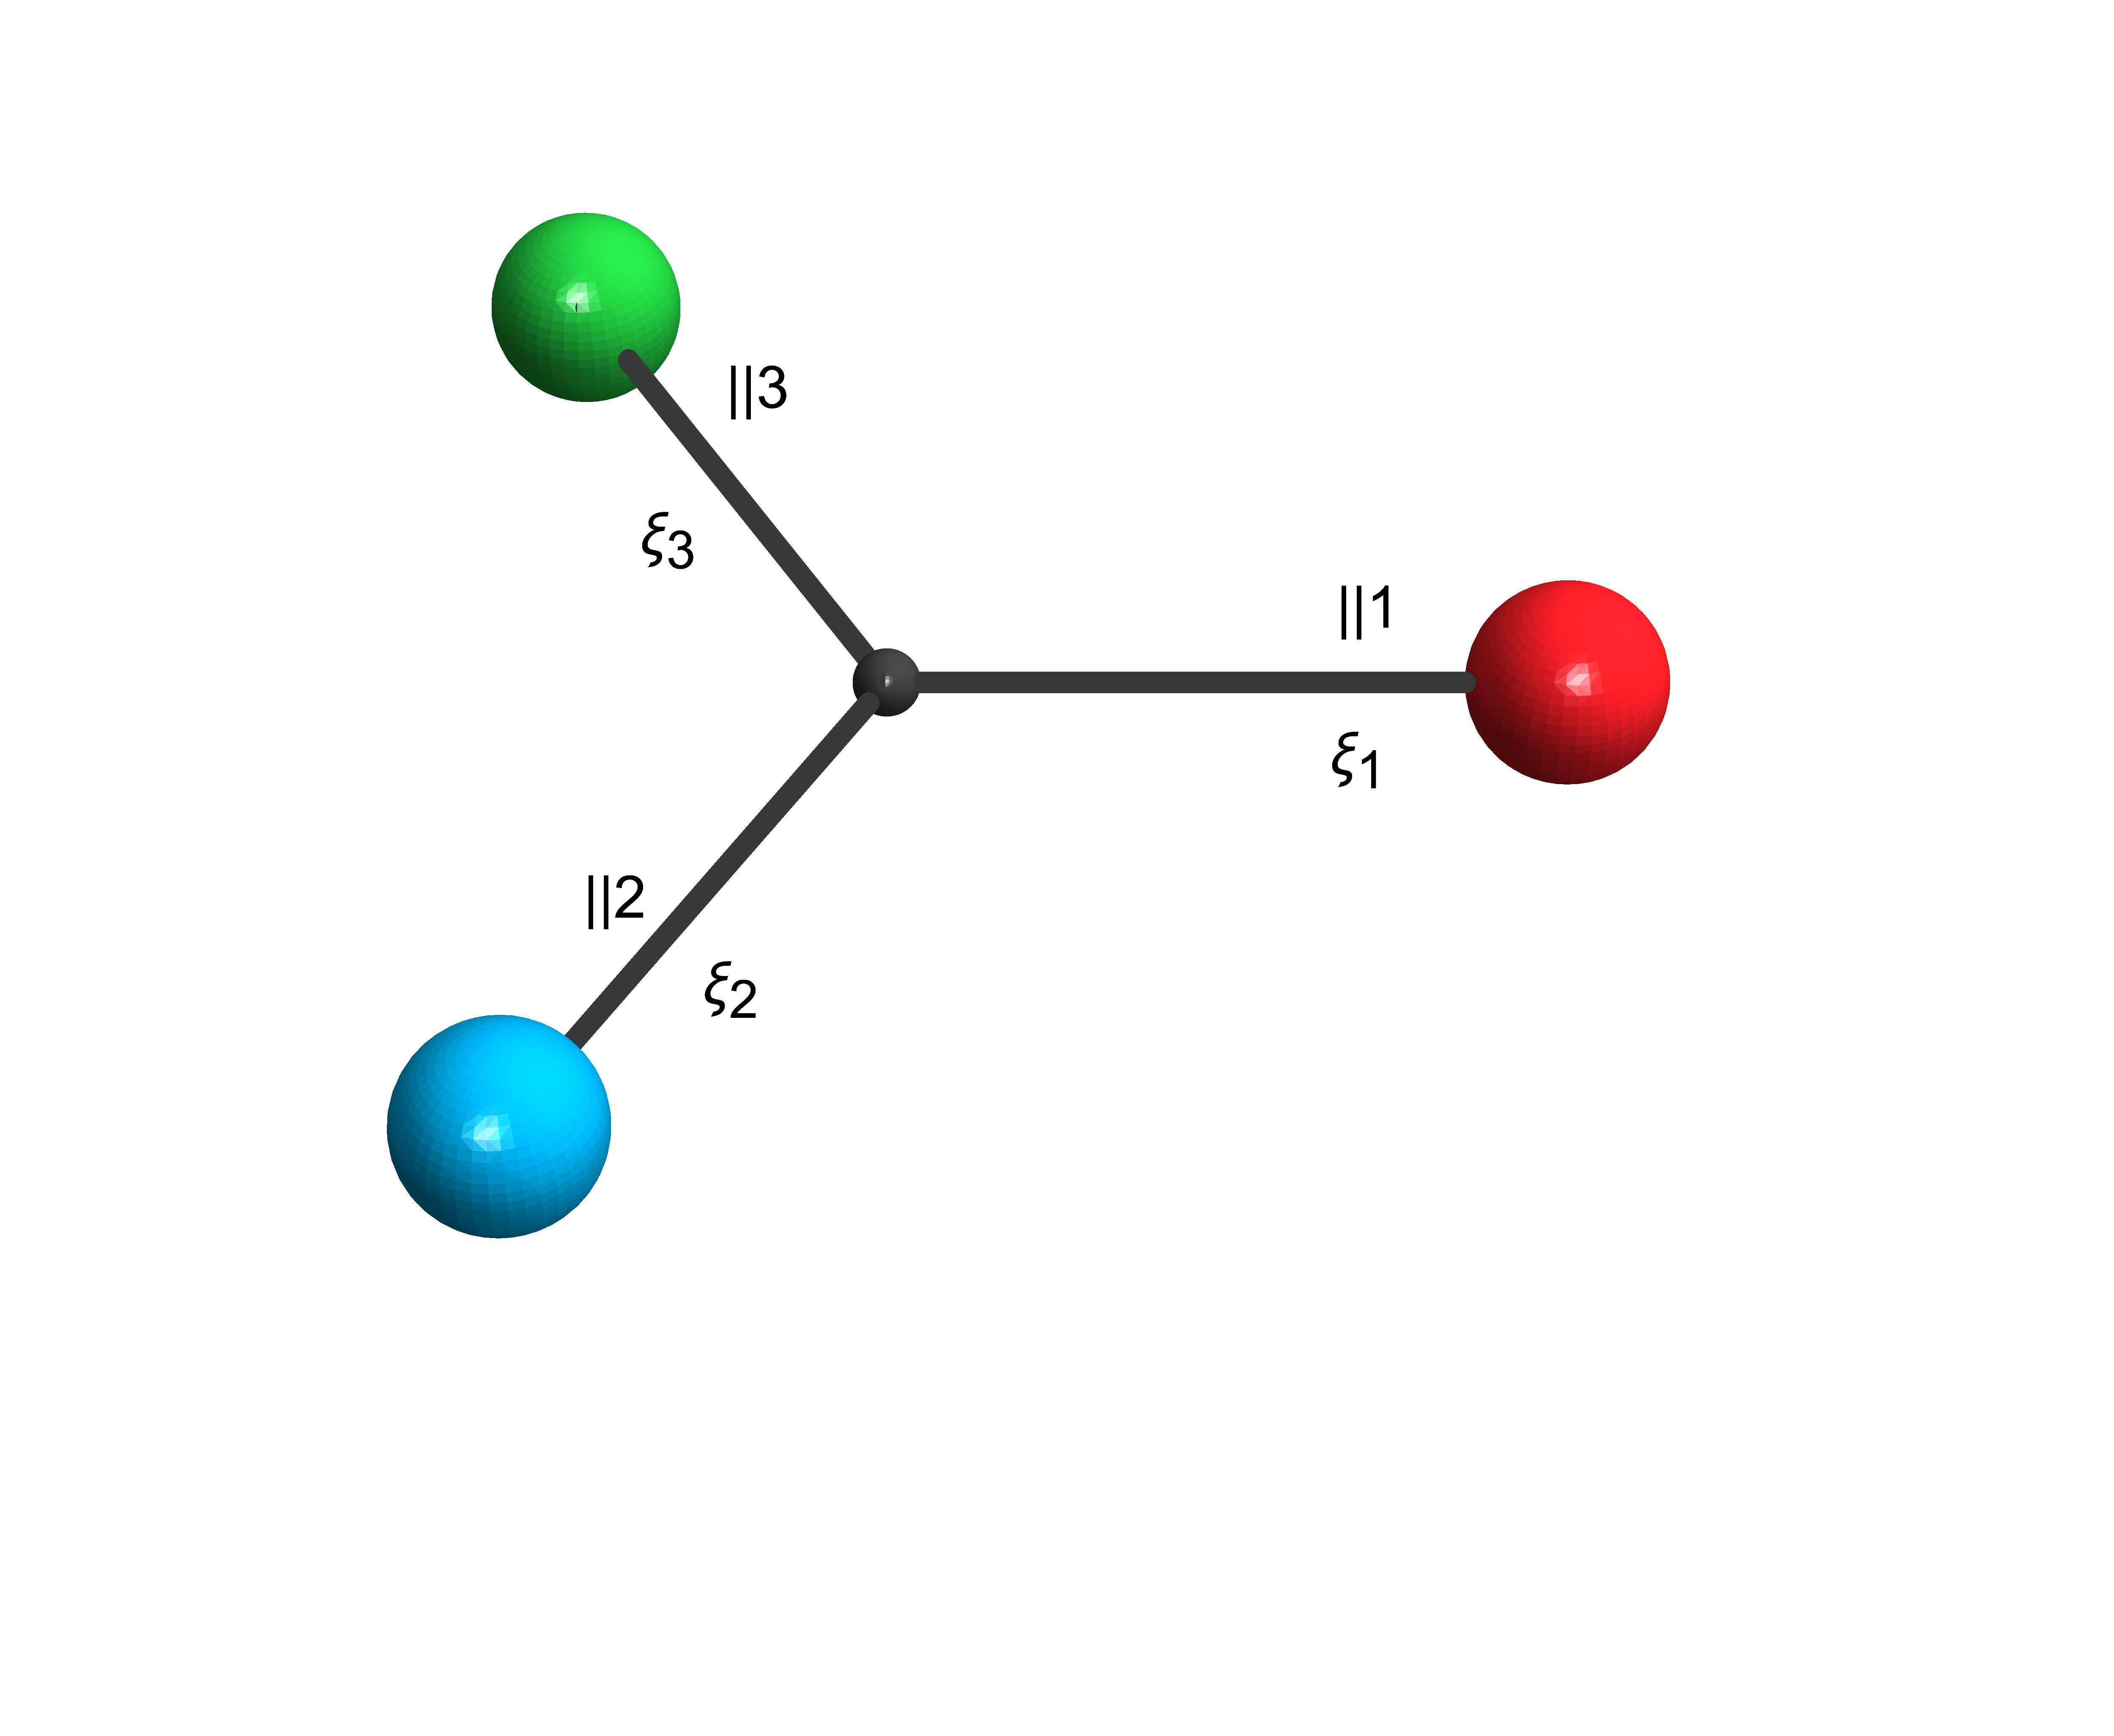
\includegraphics[scale=0.5]{/Users/philipp/Documents/GitHub/stage_cmap/images/spr3.png}
    \caption{The parking 3-sphere swimmer (\textsc{SPr3}) analyzed in \cite{Alouges2017}.}
    \label{fig:spr3}
\end{figure}

In \cite{Alouges2013}, a whole class of controllable micro-swimmer is presented. The said paper also puts forward a numerical method to address the problem of optimal swimming. However, their explicit dynamics as well as the structure of optimal swimming strokes remain largely unknown. In this paper, we will analyze further the swimmer \textsc{SPr4} from \cite{Alouges2013} and shed a light on the latter aspects. The analysis will take place very much in the spirit of the treatment of the swimmer \textsc{SPr3} in \cite{Alouges2017}, c.f. figure \ref{fig:spr3}, which originally had been presented in \cite{Alouges2013} as well. In fact, the swimmer \textsc{SPr4} is a natural generalization of the swimmer \textsc{SPr3}, capable of moving in the entire $3d$ space instead of just a plane. Although the principal techniques used in this paper are in close analogy to the ones in \cite{Alouges2017}, the more complex geometry of both the position and the shape space cause the analysis to be more involved.

Aim of this paper is to \emph{analytically} address the optimal control problem for \textsc{SPr4} in the range of \emph{small} strokes.

The rest of the paper is organized as follows: in section \ref{sec:modeling}, we give both a geometric and a kinematic description of parking 4-sphere swimmer (\textsc{SPr4}). Next, we introduce the control system treated in this paper. In section \ref{sec: symmetries}, we study the geometric structure of the control system taking advantage of the symmetries it has to satisfy due to the underlying Stokes  equations. In section \ref{sec: linearization}, we unravel the properties of the control system in the range of small strokes. Eventually, section \ref{sec: optimization} addresses the characterization of energy minimizing strokes for a special class of prescribed net displacements.






\section[Modeling]{Modeling of the swimmer as a control problem}
\label{sec:modelling}
We restrict ourselves to considering the swimmer \spr proposed in \cite{Alouges2013}. Let $(S_1, S_2, S_3, S_4)$ be a regular reference tetrahedron centered at $c \in \R^3$ such that $\dist(c, S_i) = 1$ for all $i \in \N_4$. Then the swimmer consists of four balls $(B_i)_{i \in \N_4}$ of $\R^3$ centered at $b_i \in \R^3$, all of radius $a > 0$, such that the ball $B_i$ can move along the ray starting at $c$ and passing through $S_i$. This reflects the situation where the balls are linked together by think jacks that are able to elongate. However, the viscous resistance of these jacks is neglected and therefore the fluid is assumed to permeate the entire open set $\R^3 \setminus \bigcup_{i = 1}^{4} \overline{B}_i$. The balls do not rotate around their arms which implies that the shape of the swimmer is completely determined by the four lengths $\xi_1, \xi_2, \xi_3, \xi_4$ of its arms, measured from the $c$ to the center of each ball $b_i$. However, there are no restrictions for the rotation of the swimmer around the center $c$, i.e. for fixed arm lengths, the swimmer is considered to be a rigid body in a Stokesian fluid.
Hence, the geometrical configuration of the swimmer can be described by two sets of variables:
\begin{enumerate}
	\item The vector of \emph{shape variables} $\xi := (\xi_1, \xi_2, \xi_3, \xi_4) \in \M := (\sqrt{\tfrac{3}{2}}a, +\infty)^4 \subseteq \R_+^4$, from which one obtains the relative distances $(b_{ij})_{i,j \in \N_4}$ between the balls,  where the lower bound in the open intervals is chosen such that the balls cannot overlap.
	\item The vector of \emph{position variables} $p = (c, R) \in \mathcal{P} :=  \R^3 \times \SO(3)$, which encode the global position and orientation in space of the swimmer.
\end{enumerate}
To be more precise, we consider the reference tetrahedron convexly spanned by the four unit vectors $z_1 := (2 \sqrt{2}/3,0,-1/3)$, $z_2 := (-\sqrt{2}/3,-\sqrt{2/3},-1/3)$, $z_3 := (-\sqrt{2}/3,\sqrt{2/3},-1/3)$ and $z_4 := (0,0,1)$. Position and orientation in $\R^3$ are then described by the coordinates of the center $c \in \R^3$ and the rotation $R \in SO(3)$ of the swimmer with respect to the reference orientation induced by the reference tetrahedron, i.e. if the arms are aligned with the reference tetrahedron, then this corresponds to the identity matrix $I \in \SO(3)$. Thus, we set $b_i := c + \xi_i R z_i$ for the center of the ball $B_i$.

The swimmer is completely described by the parameters $(\xi, p) \in \M \times \mathcal{P}$. Indeed, if we denote by $B_a$ the ball in $\R^3$ of radius $a$ centered at the origin, then for any $r \in \partial B_a$, the position of the current point on the $i$-th sphere of the swimmer in the state $(\xi, p)$ is given, for any $(\xi, p, r) \in \M \times \mathcal{P} \times \partial B_a$, by the function
\begin{equation}
	r_i(\xi, p, r) :=  c + R(\xi_i z_i + r).
\end{equation}
Note that the functions $(r_i)_{i \in \N_4}$ are analytic in $\M  \times \mathcal{P}$ and thus we can use them to calculate the instantaneous velocity on the $i$-th sphere $B_i$, which for any $(\xi, p, r) \in \M \times \mathcal{P} \times \partial B_a$ and every $i \in \N_4$ is given by
\begin{equation}
	u_i(\xi, p, r) = \dot{c} + \omega \times (\xi z_i + r) + R z_i \dot{\xi}_i,
\end{equation}
where $\omega$ is the axial vector associated with the skew matrix $\dot{R} R$.

In \cite{Alouges2013} it is shown that the system \spr, i.e. both the shape $\xi$ and the position $p$, is controllable only using the rate of change $\dot{\xi}$ of the shape. To do so, we have to understand how $p$ changes when we vary $\dot{\xi}$. To that end, the assumptions of \emph{self-propulsion} and \emph{negligible inertia of the swimmer} (which is equivalent to assuming a very low Reynolds number) are made. They imply that the total viscous force and torque exerted by the surrounding fluid on the swimmer must vanish. More precisely, the system can be written as
\begin{equation}
\label{eq: control system}
	\dot{p} = F(R, \xi) \dot{\xi} := \left ( \begin{array}{c}
	F_c(R, \xi) \\ 
	\hline
	F_\theta(R, \xi)
	\end{array}  \right ) \dot{\xi},
\end{equation}
where $\dot{c} = F_c(R, \xi) \dot{\xi}$ and $\dot{R} = F_\theta (R, \xi) \dot{\xi} $. 

In preparation for what follows, let us note that we have $F(R, \xi) \in \mathcal{L}(\R^4, T_{p}\mathcal{P})$ for any $R \in \SO(3)$ and $\xi \in \R^4$, where $\mathcal{L}(V, W)$ denotes the linear maps between two vector spaces $V$ and $W$. We quickly recall the fact that at any point $R \in \SO(3)$, see e.g. \cite{Hall2015} for details, we have 
\begin{equation}
	T_R \SO(3) = R^* \Skew_3(\R) = \{R M \mid M \in \Skew_3(\R)\},
\end{equation}
where $\Skew_n(\R)$ denotes the set of skew-symmetric real matrices of size $n \times n$. Hence, we have in particular that for any $R \in \SO(3)$ and $\xi \in \R^4$
\begin{equation}
\begin{aligned}
	F_c(R, \xi) \in \mathcal{L}(\R^4, \R^3) \text{ and } F_{\theta}(R, \xi) \in \mathcal{L}(\R^4, R^* \Skew_3(\R))
\end{aligned}
\end{equation}
and therefore we can express both $F_c(R, \xi)$ and $F_{\theta}(R, \xi)$ as real matrices of size $3 \times 4$ once we have chosen a basis for the corresponding tangent spaces. Indeed, one verifies quickly that $\Skew_3(\R)$ is a three-dimensional vector space over $\R$.


 In analogy to \cite{Alouges2017}, it is important to note here that the control system $F$ is independent of $c$ due to the translational invariance of the Stokes equations. However, the translational invariance is not the only symmetry property that \spr satisfies. The goal of the following section is to examine the structure of the control system $F$ in consequence of the symmetries it must satisfy being driven by the Stokes equations.































\section{Symmetries}
\label{sec: symmetries}
For any initial condition $p_0 = (c_0, R_0) \in \mathcal{P}$ and any control curve $\xi: I \subseteq \R \to \M$, with $I$ a neighborhood of zero, we denote by $\gamma(c_0, R_0, \xi): I \to \mathcal{P}$ the solution associated to the dynamical system
\begin{equation}
\label{eq:dynamical system}
\begin{aligned}
	&\dot{p} = F(R, \xi) \dot{\xi},& & p(0) := p_0,
\end{aligned}
\end{equation}
as well as $\gamma_c(c_0, R_0, \xi)$ and $\gamma_\theta(c_0, R_0, \xi)$ its projections on $\R^3$ and $\SO(3)$, respectively, such that for any $t \in I$
\begin{equation}
	\dot{\gamma}(c_0, R_0, \xi)(t) = F(\gamma_\theta(c_0, R_0, \xi)(t), \xi(t))\dot{\xi}(t).
\end{equation}

\subsection{Rotational invariance}
Rotational invariance of the Stokes equations expresses the fact that solution of the dynamical system (\ref{eq:dynamical system}) is invariant under rotations, i.e., that for any rotation $R \in \SO(3)$ we have for the spatial part of the solution
\begin{equation}
\label{eq:spatial rotational invariance}
	\gamma_c(c_0, R R_0, \xi)(t) = R \gamma_c (c_0, R_0, \xi)(t) + (I - R) c_0
\end{equation}
and for the angular part of the solution
\begin{equation}
\label{eq: angular rotational invariance}
	\gamma_\theta(c_0, R R_0, \xi)(t) =  R \gamma_\theta(c_0, R_0, \xi)(t)
\end{equation}
at any point in time $t \in I$. Eventually, we can rigorously state the following symmetry property of the control system (\ref{eq:dynamical system}) with respect to rotations:

\begin{condition}[Rotational invariance]
\label{cond:rotational invariance}
If $\gamma(c_0, R_0, \xi)$ is a solution of the control system (\ref{eq:dynamical system}), then so is $\gamma(c_0, R R_0, \xi)$ and (\ref{eq:spatial rotational invariance}) and (\ref{eq: angular rotational invariance}) hold.
\end{condition}

\begin{remark}
To follow the reasoning of \cite{Alouges2017}, the symmetry relations satisfied by \textsc{SPr4} are stated as hypotheses on the solution $\gamma$. In so doing, the results work for any control system of the form (\ref{eq: control system}) and satisfying the hypotheses we state, e.g. rotational invariance, independently of these hypotheses being guaranteed by the invariance of the Stokes equations under a certain group of transformations. 
\end{remark}
We then have
\begin{proposition}
\label{prop: rotational invariance}
Let $\xi_0 := \xi(0) \in \M$ denote the initial state of the control parameters and by $T_{\xi}\M$ the tangent space of $\M$ at $\xi$. If the control system (\ref{eq:dynamical system}) is invariant under rotations and for every $\xi \in \M$ it holds that $T_{\xi} \M \simeq \R^4$, then
\begin{equation}
	F_c(R, \xi) = R F_c(\xi) \text { and } F_\theta(R, \xi) = R F_{\theta} (R, \xi),
\end{equation}
for every $(R, \xi) \in \SO(3) \times \M$, where $F_c(\xi) := F_{c}(I, \xi)$ and $F_{\theta}(\xi) := F_{\theta}(I, \xi)$. 
\end{proposition}

\begin{proof}
On the one hand, we have by definition of the dynamical system (\ref{eq: control system}) that
\begin{equation}
	\dot{\gamma}_c(c_0, R, \xi) = F_c(\gamma_{\theta}(c_0, R, \xi), \xi) \dot{\xi}.
\end{equation}
On the other hand, using equation (\ref{eq:spatial rotational invariance}) and once more the definition of the dynamical system (\ref{eq:dynamical system}), we obtain
\begin{equation}
	\dot{\gamma}_c (c_0, R, \xi) = R  \dot{\gamma}_c(c_0, I, \xi) = 
	R F_c(\gamma_{\theta}(c_0, I, \xi), \xi) \dot{\xi}.
\end{equation}
Therefore, $F_c(\gamma_{\theta}(c_0, R, \xi), \xi) \dot{\xi} = R F_{c}(\gamma_{\theta}(c_0, I, \xi), \xi) \dot{\xi}$ for every $R \in \SO(3)$. Since $T_{\xi_0} \M \simeq \R^4$, evaluation of the preceding expression at $t = 0$ yields $F_{c}(R, \xi_0) = R F_{c}(I, \xi_0)$, as desired. The proof for $F_{\theta}$ is completely analogous and thus is omitted.
\end{proof}

\subsection{Permutation of two arms}
In this section, we investigate the effect of a swap of two arms on the generic solution of the dynamical system (\ref{eq:dynamical system}).
To that end, let $P_{ij} \in M_{4 \times 4}(\R)$ denote the permutation matrix that interchanges the $i$-th and $j$-th index of a vector, which corresponds to the swap of the arms $||i$ and $||j$, denoted by $(||i\leftrightsquigarrow ||j$), if applied to the shape space $\M$. In addition, let $S_{ij}$ denote the reflection of $\R^3$ sending arm $||i$ onto arm $||j$ in the reference orientation $I$. Geometrical inspection of the reference tetrahedron shows that $S_{ij}$ is always a reflection at a plane containing the remaining arms $||k$ and $||l$.

Before we formulate the symmetry conditions for the interchanging of two arms, we recall some results about how rotations behave under reflections. So far, we have only regarded the orientation of \textsc{SPr4} as a rotation matrix in $\SO(3)$. However, by Euler's rotation theorem to every such rotation matrix $R \in \SO(3)$ there exists a corresponding rotation vector $\omega \in \R^3$ which is collinear to the unique axis of rotation defined by $R$, i.e. $\omega$ is an eigenvector associated to the eigenvalue 1 of $R$. Its length is given by the angle of rotation around this axis. The rotation vector $\omega$ is then directly related to the rotation matrix $R$ via the map $\exp: \so(3) \to \SO(3)$, where $\so(3) = T_I \SO(3) = \Skew_3(\R)$ denotes the Lie algebra over $\SO(3)$, which we will illustrate in the following paragraphs.


It is clear that $\dim \Skew_3(\R) = 3$. In particular, if $R_1(\theta), R_2(\theta)$ and $R_3(\theta)$ denote the simple rotations around the $\hat{e}_1$-, $\hat{e}_2$- and $\hat{e}_3$-axis, where $\hat{e}_1, \hat{e}_2, \hat{e}_3$ denote the canonical basis vectors of $\R^3$, then the matrices
\begin{align}
\label{eq: L1}
	&L_1 = \frac{\dd}{\dd\theta}R_1(\theta)_{\mid \theta =0} = \left(\begin{array}{ccc}
	0 & 0 & 0 \\ 
	0 & 0 & -1 \\ 
	0 & 1 & 0
	\end{array}  \right ),\\
\label{eq: L2}
	&L_2 = \frac{\dd}{\dd\theta}R_2(\theta)_{\mid \theta =0} = \left (\begin{array}{ccc}
	0 & 0 & 1 \\ 
	0 & 0 & 0 \\ 
	-1 & 0 & 0
	\end{array}  \right ),\\
\label{eq: L3}
	&L_3 = \frac{\dd}{\dd\theta}R_3(\theta)_{\mid \theta =0} = \left (\begin{array}{ccc}
	0 & -1 & 0 \\ 
	1 & 0 & 0 \\ 
	0 & 0 & 0
	\end{array}  \right ),
\end{align}
form a basis of $\so(3)$ consisting of the infinitesimal rotations around the corresponding axes. If we now write $\textbf{L} := (L_1, L_2, L_3)^T$ and allow the slight abuse of notation
\begin{align}
	\omega \cdot \mathbf{L} = \omega_1 L_1 + \omega_2 L_2 + \omega_3 L_3,
\end{align}
we find by direct computation that $\exp(\omega \cdot \mathbf{L}) = R$. This relationship allows us to formulate the behavior of the orientation of \textsc{SPr4} under reflection and thus under permutation of two arms as we shall see later. Indeed, we have

\begin{lemma}
\label{lem:mirror image of orientation}
For any orientation of a rigid body characterized by $R \in \SO(3)$, the orientation of its mirror image under a reflection $S$ is given by
\begin{align}
	\tilde{R} = S R S.
\end{align}
\end{lemma}

\begin{proof}
Let us first consider the simple case where $S_i$ is the reflection of the $\hat{e}_i$-axis. Let $\omega$ and $\tilde{\omega}$ be the rotation vectors corresponding to $R$ and $\tilde{R}$, respectively. They are related by $\tilde{\omega} = -S_i \omega$, where the gain of the minus sign stems from the fact that rotation vectors are in fact pseudovectors. In other words, we not only reflect the axis of rotation but we also reverse the sense of rotation around the axis. It follows then from direct computation that
\begin{equation}
\label{eq: transformation of rotation axis}
 \tilde{\omega} \cdot \mathbf{L} = (-S_i\omega) \cdot \mathbf{L} = S_i(\omega \cdot \mathbf{L})S_i
\end{equation}
and thus we have
\begin{equation}
\tilde{R} = \exp(\tilde{\omega} \cdot \mathbf{L}) = \exp(S_i(\omega \cdot \mathbf{L})S_i) = S_iRS_i,
\end{equation}
as $S_i^{-1} = S_i$.

If now $S$ is an arbitrary reflection, we always find a rotation $Q \in \SO(3)$ such that $S = Q S_i Q^T$ for one of the elementary reflections $S_i$. Moreover, for any rotation $R' \in \SO(3)$ we find another $R \in \SO(3)$ such that $R' = Q R Q^T$. In particular, we have
\begin{equation}
\tilde{R}' = Q \tilde{R} Q^T = Q S_iRS_i Q^T = S R' S^T,
\end{equation}
as desired.
\end{proof}

With this lemma at hand, Stokes' equations allow us to state the following

\begin{condition}[Swap $(||i \leftrightsquigarrow ||j)$]
\label{cond:swap}
Let the initial position be $p_0 := (c_0, I)$. If $\gamma(c_0, I, P_{ij} \xi)$ is a solution of the control system (\ref{eq: control system}), then so is $\gamma(S_{ij}c_0, I, \xi)$ and the following relations hold
\begin{equation}
	\gamma_c(c_0, I, P_{ij} \xi) = S_{ij} \gamma_c(S_{ij}c_0, I, \xi)
\end{equation}
and
\begin{equation}
	\gamma_{\theta}(c_0, I, P_{ij} \xi ) = S_{ij} \gamma_{\theta} (S_{ij} c_0, I, \xi) S_{ij}.
\end{equation}
\end{condition}

\begin{figure}[h]
\centering
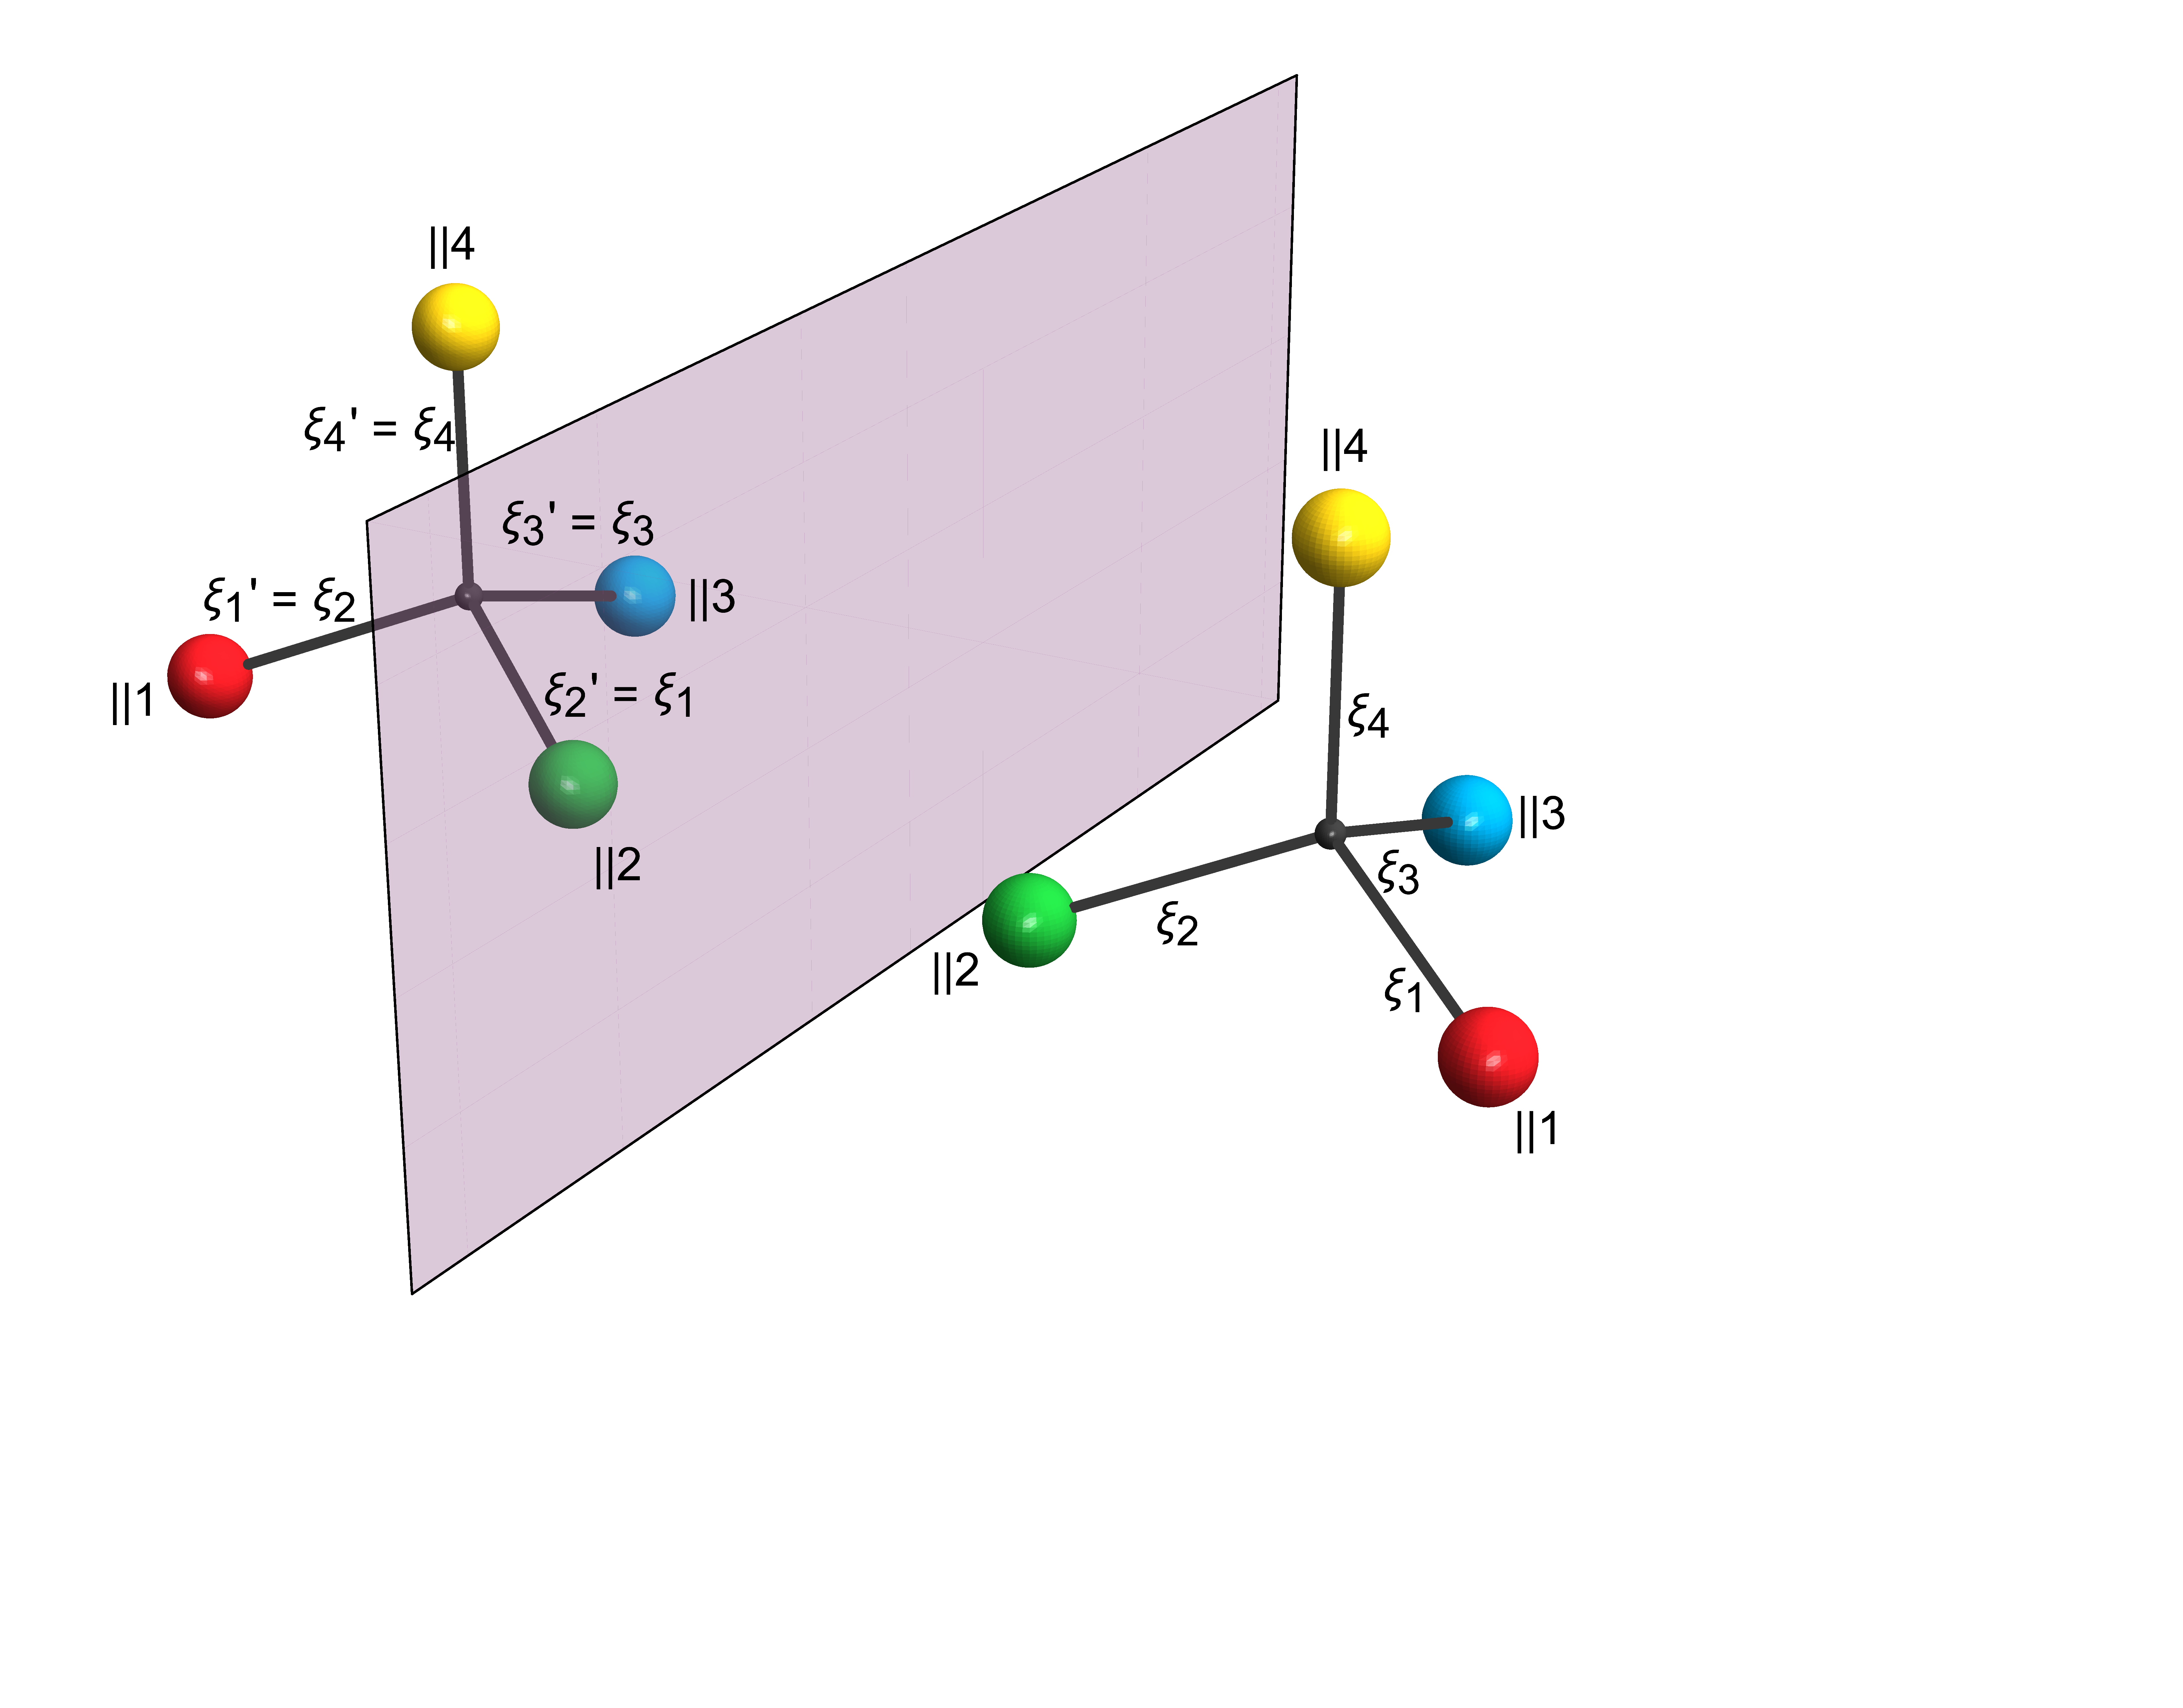
\includegraphics[width = 0.9\textwidth]{/Users/philipp/Documents/GitHub/stage_cmap/images/reflection.png}
\caption{The reflection $S_{12}$ applied to \textsc{SPr4} in the reference orientation corresponding to the swap $(||1 \leftrightsquigarrow ||2)$ }
\label{fig:reflection of swimmer}
\end{figure}

\begin{remark}
In physical terms, the previous condition stems from the invariance of Stokes equations with respect to the observation point, see figure \ref{fig:reflection of swimmer}. In fact, an observer watching the dynamics of $\gamma(S_{ij}c_0, I, \xi)$ of \textsc{SPr4} in a mirror in the reflection plane of $S_{ij}$ sees the dynamics $\gamma(c_0, I, P_{ij} \xi)$ of a micro-swimmer obtained from \textsc{SPr4} by swapping arms $||i$ and $||j$.
\end{remark}


To avoid chaos in our notation, we treat the spatial and angular parts now separately. For the spatial part, we find

\begin{proposition}
\label{prop: spatial permutation invariance}
If the control system (\ref{eq: control system}) is invariant under the swap $(||i \leftrightsquigarrow ||j)$ and $T_{\xi} \M \simeq \R^4$ for all $\xi \in \M$, then for all $\xi \in \M$
\begin{align}
	 F_c(P_{ij} \xi) = S_{ij} F_c(\xi) P_{ij}.
\end{align}
\end{proposition}

\begin{proof}
Let $\gamma_c(c_0, R_0, P_{ij} \xi)$ be the spatial part of any solution of the control problem (\ref{eq:dynamical system}). The hypothesis of rotational invariance, i.e. (\ref{eq:spatial rotational invariance}), implies that
\begin{equation}
	\gamma_c(c_0, R_0, P_{ij} \xi) = R_0 \gamma_c(c_0, I, P_{ij} \xi) + (I - R_0)c_0.
\end{equation}
From condition \ref{cond:swap}, we then get
\begin{equation}
\label{eq:spatial permutation invariance int1}
	\gamma_c(c_0, R_0, P_{ij}\xi) = R_0 S_{ij} \gamma_c(S_{ij} c_0, I, \xi) + (I - R_0)c_0.
\end{equation}
As both $\gamma_c(c_0, R_0, P_{ij} \xi)$ and $\gamma_c(S_{ij} c_0, I, \xi)$ are spatial parts of solutions of the control system (\ref{eq:dynamical system}), we have on the one hand using Proposition \ref{prop: rotational invariance}
\begin{equation}
\label{eq: spatial permutation invariance int2}
	\dot{\gamma_c}(c_0, R_0, P_{ij} \xi) = \gamma_{\theta}(c_0, R_0, P_{ij} \xi) F_c(P_{ij} \xi) P_{ij} \dot{\xi},
\end{equation}
and on the other hand using (\ref{eq:spatial permutation invariance int1}) and once more (\ref{eq:dynamical system}) together with Proposition \ref{prop: rotational invariance}
\begin{equation}
\label{eq: spatial permutation invariance int3}
	\dot{\gamma_c}(c_0, R_0, P_{ij} \xi) = R_0 S_{ij} \dot{\gamma}_c(S_{ij} c_0, I, \xi) = R_0 S_{ij} \gamma_\theta(S_{ij} c_0, I, \xi) F_c(\xi) \dot{\xi}.
\end{equation}
Equating (\ref{eq: spatial permutation invariance int2}) and (\ref{eq: spatial permutation invariance int3}) at $t = 0$ yields $ F_c(P_{ij} \xi_0) = S_{ij} F_c(\xi_0) P_{ij}$, since by hypothesis $T_{\xi_0} \M \simeq \R^4$. As $\xi_0$ was arbitrary, we conclude.
\end{proof}

For the angular part, we first have to choose a basis and fix some notation. Naturally, we choose the canonical basis $\mathcal{E} := (e_1, e_2, e_3, e_4)$ for $\R^4$. For $\so(3)$, we choose the basis $\mathcal{L} := (L_1, L_2, L_3)$, where the matrices $L_i$ are defined in (\ref{eq: L1}) - (\ref{eq: L3}). Then we denote the matrix representing an arbitrary linear map $T: V \to W$ between two vector spaces $V$ and $W$ with respect to two bases $\mathcal{B}$ and $\mathcal{B}'$ by $[T]_{\mathcal{B}}^{\mathcal{B}'}$. Subsequently, we will especially make use of the adjoint map on $\so(3)$ associated to an orthogonal transformation $Q$ of $\R^3$. More precisely, if $Q$ is an orthogonal transformation of $\R^3$, we define the adjoint map $\ad_Q : \so(3) \to \so(3)$ by
\begin{equation}
\ad_Q(M) := Q M Q^T,
\end{equation}
which is clearly a linear map.

Thus, before we address the invariance property of the angular part of the control system under a swap of arms, let us prove the following

\begin{lemma}
\label{lem:representation matrix of adjoint of reflection}
Let $S: \R^3 \to \R^3$ be an arbitrary reflection at a plane. Then the representation matrix of the adjoint map $\ad_S$ is given by $[\ad_S]_{\mathcal{L}} = -S$.
\end{lemma}


\begin{proof}
We have already seen in the proof of Lemma \ref{lem:mirror image of orientation} that for the reflection $S_i$ of the $\hat{e}_i$-axis, we have $[\ad_{S_i}]_{\mathcal{L}} = -S_i$. Moreover, by direct calculation, we find for the elementary rotations $R_i(\theta)$ that $[\ad_{R_i(\theta)}]_{\mathcal{L}} = R_{i}(\theta)$. Now if $S$ is an arbitrary reflection, we find $Q \in SO(3)$ such that $S = Q S_i Q^T$ for one of the elementary reflections $S_i$. In particular, we find by Euler's rotation theorem three angles $\alpha, \beta, \gamma \in \R$ such that $Q = R_{3}(\gamma) R_{2}(\beta) R_{1}(\alpha)$ and therefore
\begin{equation}
\ad_Q = \ad_{R_3(\gamma)} \circ \ad_{R_{2}(\beta)} \circ \ad_{R_{1}(\alpha)},
\end{equation}
which implies that $[\ad_{Q}]_{\mathcal{L}} = Q$. Since we clearly have $\ad_{Q}^{-1} = \ad_{Q^{-1}} = \ad_{Q^T}$, we have $[\ad_{Q^T}]_{\mathcal{L}} = Q^T$. Hence, due to $\ad_S = \ad_Q \circ \ad_{S_i} \circ \ad_{Q^T}$, we find
\begin{equation}
[\ad_S]_{\mathcal{L}} = - Q S_i Q^T = -S,
\end{equation}
as desired.
\end{proof}

\begin{proposition}
\label{prop: angular permutation invariance}
If the control system (\ref{eq:dynamical system}) is invariant under the swap $(||i \leftrightsquigarrow ||j)$ and $T_{\xi}\M \simeq \R^4$ for all $\xi \in \M$, then for all $\xi \in \M$
\begin{equation}
[F_{\theta}(P_{ij} \xi)]_{\mathcal{E}}^{\mathcal{L}} = - S_{ij} [F_{\theta}(\xi)]_{\mathcal{E}}^{\mathcal{L}} P_{ij}.
\end{equation}
\end{proposition}

\begin{proof}
Let $\gamma_\theta(c_0, R_0, P_{ij}\xi)$ be the angular part of any solution of the control problem (\ref{eq:dynamical system}). By the rotational invariance hypothesis, i.e. (\ref{eq: angular rotational invariance}), we have
\begin{equation}
	\gamma_\theta(c_0, R_0, P_{ij}\xi) = R_0 \gamma_\theta(c_0, I, \xi).
\end{equation}
Then Condition \ref{cond:swap} implies that
\begin{equation}
\label{eq: angular permutation invariance int1}
	\gamma_\theta(c_0, R_0,P_{ij} \xi) = R_0 S_{ij} \gamma_\theta(S_{ij}c_0, I, \xi) S_{ij}.
\end{equation}
Since both $\gamma_\theta(c_0, R_0, P_{ij} \xi)$ and $\gamma_\theta(S_{ij} c_0, I, \xi)$ are the angular parts of solutions of the control problem (\ref{eq:dynamical system}), we obtain with Proposition \ref{prop: rotational invariance} on the one hand
\begin{equation}
\label{eq: angular permutation invariance int2}
	\dot{\gamma_\theta}(c_0, R_0, P_{ij} \xi)= \gamma_\theta(c_0, R_0, P_{ij} \xi) F_{\theta}(P_{ij} \xi) P_{ij } \dot{\xi}
\end{equation}
and on the other hand using (\ref{eq: angular permutation invariance int1}) and once more Proposition \ref{prop: rotational invariance}
\begin{equation}
\label{eq: angular permutation invariance int3}
	\dot{\gamma_\theta}(c_0, R_0, P_{ij} \xi) =  R_0 S_{ij} \dot{\gamma_\theta}(S_{ij} c_0, I, \xi) S_{ij} = R_0 S_{ij} \gamma_\theta(S_{ij} c_0, I, \xi) F_{\theta}(\xi) \dot{\xi} S_{ij}.
\end{equation}
Imposing equality of (\ref{eq: angular permutation invariance int2}) and (\ref{eq: angular permutation invariance int3}) at $t = 0$ yields
\begin{equation}
	F_{\theta}(P_{ij} \xi_0) P_{ij}  \dot{\xi}(0) = S_{ij} F_{\theta}(\xi_0) \dot{\xi}(0) S_{ij}.
\end{equation}
By choice of the canonical basis for $\R^4$ we clearly have $[P_{ij}]_{\mathcal{E}}^{\mathcal{E}} = P_{ij}$. Therefore, by Lemma \ref{lem:representation matrix of adjoint of reflection}, we have
\begin{equation}
	[F_{\theta}(P_{ij} \xi_0)]_{\mathcal{E}}^{\mathcal{L}}  P_{ij} [\dot{\xi}(0)]_{\mathcal{E}} = [S_{ij} F_{\theta}(\xi_0) \dot{\xi}(0) S_{ij}]_{\mathcal{L}} = -S_{ij} [F_{\theta}(\xi_0)]_{\mathcal{E}}^{\mathcal{L}} [\dot{\xi}(0)]_{\mathcal{E}}.
\end{equation}
Recalling that $T_{\xi_0} \M \simeq \R^4$ as well as the arbitrariness of $\xi_0$ finish the proof.
\end{proof}

In the following sections, we will always understand $F_{\theta}(\xi)$ as a matrix of size $3 \times 4$ and thus, since no confusion may arise, we will abandon the slightly cumbersome notation and identify $[F_{\theta}(\xi)]_{\mathcal{E}}^{\mathcal{L}}$ with $F_{\theta}(\xi)$.







\section[The small strokes regime]{The small strokes regime}
\label{sec: linearization}
Let us return to the control equations for \textsc{SPr4} given by (\ref{eq:dynamical system}). The response of the control system is characterized by the two matrix valued functions $F_c, F_{\theta}: \SO(3) \times \R^4 \to M_{3 \times 4}(\R)$ which can by Proposition \ref{prop: rotational invariance} can be factorized as:
\begin{equation}
\label{eq: reminder control system}
	F_{c}(R, \zeta) = R F_{c}(\zeta) \text{ and } F_{\theta}(R, \xi) = R F_{\theta}(\zeta),
\end{equation}
with $F_{c}(\zeta) := F_c(I, \zeta)$ and $F_{\theta}(\zeta) := F_{\theta}(I, \zeta)$. Hereinafter, we suppose that $\zeta := \xi_0 + \xi$ with $\xi_0 \in \M$ having all its components equal. Furthermore, we set $F_{c, \xi_0}(\xi) := F_{c}(\xi_0 + \xi)$ and analogously $F_{\theta, \xi_0}(\xi) := F_{\theta}(\xi_0 + \xi)$. It has been shown in \cite{Alouges2013} that $F$ and thus both $F_{ c, \xi_0}$ and $F_{\theta, \xi_0}$ are analytic functions. Therefore, we can consider their first order expansions in $\xi$:
\begin{align}
\label{eq: spatial control expansion}
	F_{c, \xi_0}(\xi)\eta &= F_{c, 0} \eta  + \h_{c,0}(\xi \otimes \eta) + \mathcal{O}(|\xi|)\eta\\
\label{eq: angular control expansion}
	F_{\theta, \xi_0}(\xi) \eta &= F_{\theta, 0} \eta + \h_{\theta, 0}(\xi \otimes \eta) + \mathcal{O}(|\xi|)\eta,
\end{align}
where $F_{c,0} := F_{c}(\xi_0) \in M_{3 \times 4}(\R)$, $\h_{c,0}\in \mathcal{L}(\R^4 \otimes \R^4, \R^3)$ represents the first order derivative of $F_{c, \xi_0}$ at $\xi = 0$ and for $F_{\theta, \xi}$ the analogous definitions are made.
The purpose of this section is to reveal the structure of the different terms in the expansions (\ref{eq: spatial control expansion}) and (\ref{eq: angular control expansion}) in light of the symmetry properties fulfilled by $F_{c}$ and $F_{\theta}$ due to Propositions \ref{prop: spatial permutation invariance} and \ref{prop: angular permutation invariance} , i.e.
\begin{align}
\label{eq: spatial and angular first order expansion}
	F_{c}(P_{ij} \xi) = S_{ij} F_{c}(\xi) P_{ij}& & \text{ and } & & 			F_{\theta}(P_{ij} \xi) = - S_{ij} F_{\theta}(\xi) P_{ij} & & \forall \xi \in \M.
\end{align}

The following slightly generalized statement of Lemma 9 in \cite{Alouges2017} proves useful in our case as well. However, the proof, being exactly the same, is omitted.

\begin{lemma}
\label{lem: general symmetries of expansion terms}
Let $G: \R^n \to M_{m \times n}(\R)$ be an analytic function and $S \in M_{m \times m}(\R)$ and $P \in M_{n \times n}(\R)$ matrices such that $G(P \xi) = S G(\xi) P$ for every $\xi \in \R^n$. For $\xi_0 \in \R^n$ with all components equal, set $G_{\xi_0}(\xi) := G(\xi_0 + \xi)$ and write the first order expansion
\begin{equation}
	G_{\xi_0}(\xi)\eta = G_0 \eta + \h_0(\xi \otimes \eta) + \mathcal{O}(|\xi|)\eta.
\end{equation}
Then we have
\begin{equation}
	G_0 = S G_0 P,
\end{equation}
and
\begin{eqnarray}
	\h_0((P \xi) \otimes \eta) = S \h_0(\xi \otimes (P \eta)) &  & \forall \xi, \eta \in \R^n.
\end{eqnarray}
\end{lemma}

\subsection{The zeroth order terms $F_{c,0}$ and $F_{\theta, 0}$} 
One could directly use Lemma \ref{lem: general symmetries of expansion terms} to obtain the terms of order zero up to a scalar by solving a system of two matrix equations as it was done in \cite{Alouges2017}. Yet, there is a direct geometric argument, which incidentally also works for \textsc{SPr3} in \cite{Alouges2017},  that reveals their structure.
Let us denote by $A^{(i)}$ the $i$-th column of a matrix $A \in M_{m \times n}(\R)$. Then we note that for the spatial term $F_{c,0}$ and any $i \in \N_4$ we obtain from Lemma \ref{lem: general symmetries of expansion terms} and Proposition \ref{prop: spatial permutation invariance}
\begin{equation}
\label{eq:zeroth spatial term condition 1}
	F_{c,0}^{(i)} = F_{c,0} e_i = S_{ij} F_{c,0} P_{ij} e_i = S_{ij} F_{c,0} e_j = S_{ij} F_{c,0}^{(j)}.
\end{equation}
Similarly, for any $k \in \N_4$ one has
\begin{equation}
\label{eq:zeroth spatial term condition 2}
F_{c,0}^{(k)} = S_{ij} F_{c,0} P_{ij} e_k = S_{ij} F_{c,0} e_k = S_{ij} F_{c,0}^{(k)}.
\end{equation}
Recall that $S_{ij}$ is the reflection that maps the arm $||i$ onto arm $||j$ and vice-versa in the reference orientation, i.e. where $||i$ is collinear to $z_i$, the $i$-th arm of the reference tetrahedron defined in section \ref{sec:modeling}. In particular, the plane of reflection is defined by the origin and the remaining arms of the reference tetrahedron, i.e. by the vectors $z_k$ and $z_l$. Thus, equation (\ref{eq:zeroth spatial term condition 2}) implies that $F_{c,0}^{(k)} \in \Span\{z_k, z_l\}$ as $F_{c,0}^{(k)}$ apparently is an eigenvector associated to the eigenvalue 1 of $S_{ij}$. Yet, the same argument shows that $F_{c,0}^{(k)} \in \Span\{z_k, z_i\}$ and $F_{c,0} \in \Span\{z_k, z_j\}$ and the vectors $z_i, z_j$ and $z_l$ being linearly independent implies that $F_{c,0}^{(k)} = a_k z_k$ for some $a_k \in \R$. Due to equation (\ref{eq:zeroth spatial term condition 1}) and the fact that $S_{ij}$ is orthogonal, we have $|a_i| = |a_j| = |a_k| = |a_l|$. Finally, we note that the quantity $a_k z_k \cdot z_k$ stays constant under change of indices again in consequence of the symmetry conditions from Lemma \ref{lem: general symmetries of expansion terms}. Hence, we have $a_1 = a_2 = a_3 =a_4 := \mathfrak{a}$ and therefore
\begin{equation}
	F_{c,0} = \mathfrak{a} (z_1 |z_2| z_3|z_4).
\end{equation}

In the following sections, we will exploit the orthonormal basis of $\R^4$ consisting of the vectors $\tau_1 : = \tfrac{1}{\sqrt{6}}(-2,1,1,0)^T$, $\tau_2 := \tfrac{1}{\sqrt{2}}(0,1,-1,0)^T$, $\tau_{3}:= \tfrac{1}{2 \sqrt{3}} (1,1,1,-3)^T$ and $\tau_4:= \tfrac{1}{2}(1,1,1,1)^T$, in terms of which $F_{c,0}$ can be written as $F_{c, 0} = -3 \sqrt{3} \mathfrak{a} [\tau_1|\tau_2| \tau_3 ]^T$.

For the angular term $F_{\theta,0}$ we find by Lemma \ref{lem: general symmetries of expansion terms}, Proposition \ref{prop: angular permutation invariance} and a similar argument for any $k \in \N_4$ that
\begin{equation}
F_{\theta, 0}^{(k)} = -S_{ij} F_{\theta, 0}^{(k)}.
\end{equation}
This means that in this case $F_{\theta,0}^{(k)}$ is an eigenvector to the eigenvalue $-1$ and therefore must be orthogonal to the plane of reflection, i.e. $\Span\{z_k, z_l\}$. The same is true for the reflections $S_{il}$ and $S_{jl}$ and hence $F_{c,0}^{(k)}$ is in particular orthogonal to $z_i, z_j, z_l$. This eventually implies that $ F_{\theta, 0} = 0$ since the latter three vectors form a basis of $\R^3$.

\begin{remark}
First, we observe that the upper left corner of $F_{c,0}$ corresponding to the arms $||1, ||2$ and $||3$ up to multiplication by a scalar is the same as for \textsc{SPr3} in \cite{Alouges2017}. Furthermore, one notes that physically it is  clear that $F_{\theta,0}$ must vanish since by hypothesis $\xi_0$ has all its components equal and thus the swimmer is in a symmetric shape at $\xi = 0$. Therefore, the balls moving along their axes cannot create any torque.
\end{remark}


%However, setting $\mathfrak{a} := -3/\sqrt{2} a$ yields the slightly more convenient form
%\begin{equation}
%	F_{c, 0}  = \left ( \begin{array}{cccc}
%	- 2 \mathfrak{a}  & \mathfrak{a}  & \mathfrak{a}  & 0 \\ 
%	0 & \sqrt{3}\mathfrak{a}  & -\sqrt{3}\mathfrak{a}  & 0 \\ 
%	 \tfrac{1}{\sqrt{2}}\mathfrak{a} & \tfrac{1}{\sqrt{2}}\mathfrak{a} & \tfrac{1}{\sqrt{2}} \mathfrak{a}  & \tfrac{-3}{\sqrt{2}}\mathfrak{a} 
%	\end{array} \right ) \text{ with } \mathfrak{a} \in \R.
%\end{equation}
%One recognizes in the top left corner of $F_{c,0}$ the zeroth order term of the control system associated to the swimmer \textsc{SPr3} in \cite{Alouges2017}. Further

%By applying Lemma \ref{lem: general symmetries of expansion terms} to $F_{c, \xi_0}$ and $F_{\theta, \xi_0}$, we obtain two linear systems of matrix equations in the unknowns $F_{c, 0}$ and $F_{\theta,0}$. To solve these two systems, we eventually have to determine at least some of the matrices $S_{ij}$. Let $S_{kl}(\phi)$ denote the reflection at the plane orthogonal to the $\hat{e}_k-\hat{e}_l$-plane making an angle of $\phi$ with the $\hat{e}_k$-axis. By geometrical inspection of the reference tetrahedron $(S_1, S_2, S_3, S_4)$, we find that
%\begin{eqnarray}
%	S_{12} = S_{12}\left (\tfrac{2\pi}{3}\right ), & S_{23} = S_{12}(0),  & S_{13} = S_{13}\left (\tfrac{\pi - \alpha_{\mathrm{tet}}}{2}\right ),
%\end{eqnarray}
%where $\alpha_{\mathrm{tet}} = \arccos (-1/3)$ denotes the angle between two legs of a regular tetrahedron. Indeed, it happens that these three matrices are enough to determine both terms of order and one finds that $F_{\theta, 0} = 0$ and


%\begin{remark}
%First, we observe that the upper left corner of $F_{c,0}$ corresponding to the arms $||1, ||2$ and $||3$ is exactly the same as for \textsc{SPr3} in \cite{Alouges2017}. Furthermore, one notes that physically it is  clear that $F_{\theta,0}$ must vanish since by hypothesis $\xi_0$ has all its components equal and thus the swimmer is in a symmetric shape at $\xi = 0$. Therefore, the balls moving along their axes cannot create any torque. Lastly, one should note that apparently $F_{c,0} \sim (z_1 |z_2|z_3|z_4)$ which can be shown directly using the symmetry properties.
%\end{remark}

\subsection{The first order terms $\h_{c,0}$ and $\h_{\theta,0}$}
Following the approach in \cite{Alouges2017}, we evaluate the tensors $\h_{c,0}$ and $\h_{\theta,0}$ on the basis $(e_{i} \otimes e_{j})_{i,j \in \N_4}$. Setting $A_k := (\h_{c,0}(e_i \otimes e_j)\cdot \hat{e}_k)_{i,j \in \N_4}$ and $B_k:= (\h_{\theta,0}(e_i \otimes e_j)\cdot L_k)_{i,j \in \N_4}$ for $k \in \N_3$, we can write the vectors $\h_{c,0}(\xi \otimes \eta), \h_{\theta,0}(\xi \otimes \eta) \in \R^3$ for any $\xi, \eta \in \R^3$ as
\begin{equation}
\label{eq: matrix representation of spatial first order term}
	\h_{c,0}(\xi \otimes \eta) = \sum_{k \in \N_3}(A_k \eta \cdot \xi)\hat{e}_k, 
\end{equation}
and similarly
\begin{equation}
\label{eq: matrix representation of angular first order term}
	\h_{\theta, 0}(\xi \otimes \eta) = \sum_{k \in \N_3}(B_k \eta \cdot \xi) L_k.
\end{equation}

We could pursue the approach of \cite{Alouges2017} and directly calculate the matrices $A_k$ and $B_k$. However, as we shall see later, the dynamics of \textsc{SPr4}, up to higher order terms in the norm of the control curve $\xi$, will only be governed by their skew symmetric parts. Thus, we will evade this strenuous task and we determine the skew symmetric matrices $M_k := \tfrac{1}{2}(A_k - A_k^T)$ and $M_{k + 3}:= \tfrac{1}{2}(B_k - B_k^T)$ for $k \in \N_3$, up to two scalar parameters, using a geometric argument similar to the one used in the previous section. Nevertheless, it is possible to calculate the symmetric parts of the matrices $A_k$ and $B_k$ using similar geometric arguments, c.f. appendix, to obtain a complete description of the dynamics.


To that end, we notice that Lemma \ref{lem: general symmetries of expansion terms} together with the fact that $(P_{ij})^2 = I$ yields for all $i,j \in \N_4$ and for all $\xi, \eta \in \N_4$
\begin{equation}
	S_{ij} \h_{c,0}(P_{ij} \xi \otimes P_{ij} \eta) = \h_{c,0}(\xi \otimes \eta),
\end{equation}
as well as
\begin{equation}
	-S_{ij} \h_{\theta,0}(P_{ij} \xi \otimes P_{ij} \eta) = \h_{\theta, 0}(\xi \otimes \eta).
\end{equation}
Next, we define $\mathcal{K}_{c,0}(\xi \otimes \eta) := \tfrac{1}{2}[\h_{c,0}(\xi \otimes \eta) - \h_{c,0}(\eta \otimes \xi)]$ and similarly $\mathcal{K}_{\theta,0}$ such that
\begin{equation}
	M_k = (\mathcal{K}_{c,0}(e_i \otimes e_j) \cdot \hat{e}_k)_{i,j \in \N_4} \text{ and } M_{k + 3} = (\mathcal{K}_{\theta,0}(e_i \otimes e_j) \cdot L_k)_{i,j \in \N_4},\;\; k \in \N_3.
\end{equation} 
In particular, it is clear that $\mathcal{K}_{c,0}$ and $\mathcal{K}_{\theta,0}$ satisfy the same symmetry relations as $\h_{c,0}$ and $\h_{\theta, 0}$, respectively, and additionally, we have $\mathcal{K}_{c,0}(e_i \otimes e_j) = - \mathcal{K}_{c,0}(e_j \otimes e_i)$ and $\mathcal{K}_{\theta,0}(e_i \otimes e_j) = - \mathcal{K}_{\theta,0}(e_j \otimes e_i)$.

For the spatial part, we deduce from the symmetry properties above that for all $i, j \in \N_4$	
\begin{equation}
	\K_{c,0}(e_i \otimes e_j) = S_{ij} \K_{c,0}(e_j \otimes e_i) = -S_{ij} \K_{c,0}(e_i \otimes e_j)
\end{equation}
and therefore $\K_{c,0}(e_i \otimes e_j)$ is an eigenvector associated to the eigenvalue $-1$ of the reflection $S_{ij}$. The reflection $S_{ij}$ taking place at the plane passing through the two remaining arms of the reference tetrahedron $z_k$ and $z_l$, implies that $\K_{c,0}(e_i \otimes e_j) = \alpha_{ij}( z_k \times z_l)$ for some scalar $\alpha_{ij} \in \R$. Additionally, we have $\K_{c,0}(e_i \otimes e_j) = S_{jk} \K_{c,0}(e_i \otimes e_k) = \alpha_{ik}(z_j \times z_l)$ and since $S_{jk}$ is orthogonal, we have $|\alpha_{ij}| = |\alpha_{ik}|$ as the vectors $z_i$ are normalized. Eventually, one quickly verifies that the quantity
\begin{equation}
	\K_{c,0}(e_i \otimes e_j) \cdot \sgn(ijkl) (z_k \times z_l),
\end{equation}
where $\sgn(ijkl)$ denotes the parity of the permutation $(ijkl)$ of $\N_4$, stays constant under any permutation of the indices as well as any symmetry condition. Hence, we may conclude that
\begin{equation}
	\K_{c,0}(e_i \otimes e_j) = \alpha \sgn(ijkl) (z_k \times z_l),
\end{equation}
for all $i \neq j \in \N_4$ and some scalar $\alpha \in \R$. Clearly, the symmetry conditions imply that $\K_{c,0}(e_i \otimes e_i) = 0$ for all $i \in  \N_4$. Thus, we have determined the matrices $M_1, M_2, M_3$ up to one scalar parameter. By explicitly calculating the cross products $z_i \times z_j$, we find
\renewcommand{\arraystretch}{1.1}
\begin{align}
\label{eq: M1 and M2}
M_1 = \alpha \left ( \begin{array}{cccc}
0 & 3 & 3 & 2 \\ 
-3 & 0 & 0 & -1 \\ 
-3 & 0 & 0 & -1 \\ 
-2 & 1 & 1 & 0
\end{array} \right ) &, &
M_2 = \sqrt{3} \alpha \left (
\begin{array}{cccc}
0 & 1 & -1 & 0 \\ 
-1 & 0 & -2 & -1 \\ 
1 & 2 & 0 & 1 \\ 
0 & 1 & -1 & 0
\end{array} \right),
\end{align}
and
\begin{align}
\label{eq: M3}
M_3 = 2 \sqrt{2} \alpha \left (
\begin{array}{cccc}
0 & 0 & 0 & -1 \\ 
0 & 0 & 0 & -1 \\ 
0 & 0 & 0 & -1 \\ 
1 & 1 & 1 & 0
\end{array} 
\right ).
\end{align}
Similarly, for the angular part, we find that
\begin{equation}
	\K_{\theta, 0}(e_i \otimes e_j) = - S_{kl} \K_{\theta,0}(e_i \otimes e_j)
\end{equation}
and therefore $\K_{\theta,0}(e_i \otimes e_j) = \delta_{ij} e_i \times e_j$. By noticing that this time the quantity $\K_{\theta,0}(e_i \otimes e_j) \cdot (z_i \times z_j)$ stays constant, a similar argument to the one above shows that
\begin{equation}
\K_{\theta,0}(e_i \otimes e_j) = \delta (z_i \times z_j),
\end{equation}
for all $i \neq j \in \N_4$. Again, we have $\K_{\theta}(e_i \otimes e_i) = 0$ for all $i \in \N_4$. A calculation similar to the one above now yields
\begin{align}
\label{eq: M4 and M5}
	M_4 = \delta \left (
	\begin{array}{cccc}
	0 & 1 & -1 & 0 \\ 
	-1 & 0 & -2 & 3 \\ 
	1 & 2 & 0 & -3 \\ 
	0 & -3 & 3 & 0
	\end{array} 
	\right ) &, & M_5 = \sqrt{3} \delta \left ( \begin{array}{cccc}
	0 & -1 & -1 & 2 \\ 
	1 & 0 & 0 & -1 \\ 
	1 & 0 & 0 & -1 \\ 
	-2 & 1 & 1 & 0
	\end{array} \right ) ,
\end{align}
and
\begin{align}
\label{eq: M6}
M_6 = 2 \sqrt{2} \delta \left (\begin{array}{cccc}
0 & 1 & -1 & 0 \\ 
-1 & 0 & 1 & 0 \\ 
1 & -1 & 0 & 0 \\ 
0 & 0 & 0 & 0
\end{array}  \right ).
\end{align}

\begin{remark}
At this point, let us point out the apparent similarity between the matrices $M_1, M_2$ and $M_6$ with their corresponding matrices in \cite{Alouges2017}. In fact, in the upper left corner, i.e. the entries that relate the first three arms to each other, we retrieve the same matrices as in \cite{Alouges2017} up to rescaling $\alpha$ and $\delta$, which very well reflects the similarity between \textsc{SPr3} and \textsc{SPr4}. However, the fact that it is the first three arms that corresponds to the three arms in \textsc{Spr3} merely stems from our choice of the reference orientation.
\end{remark}

\subsection{The linearized control equations}
Herein, we denote by $J$ the closed interval  $[0,2\pi] \subset \R$ and we define the so-called \emph{strokes space} as $H_\sharp^1(J, \R^4)$, i.e. the Sobolev space of $2\pi$-periodic vector valued functions of $L_{\sharp}^2(J, \R^4)$ having first order weak derivative in $L_{\sharp}^2(\R^4)$. For every $f \in L^{2}_{\sharp}(J, \R^4)$ we denote by $\langle f \rangle := (2\pi)^{-1} \int_{J} f(s) \dd s$ the average of $f$ on $J$.

In the previous section, we have seen that the control system governing the evolution of \textsc{SPr4} under the action of the control parameters $\zeta \in \M$ is given by
\begin{align}
\begin{cases}
	\dot{c} &= R F_c(\zeta) \dot{\zeta}\\
	\dot{R} &= R F_{\theta}(\zeta) \dot{\zeta},
\end{cases}
\end{align}
where $(c,R) \in \mathcal{P} = \R^3 \times \SO(3)$, the systems $F_{c}, F_{\theta}: \M \to M_{3 \times
 4}(\R)$ are given by (\ref{eq: reminder control system}) and $\dot{\zeta}  \in T_{\zeta}\M$. Furthermore, we have seen previously, c.f. (\ref{eq: spatial and angular first order expansion}), (\ref{eq: matrix representation of spatial first order term}) and (\ref{eq: matrix representation of angular first order term}), that if we set $\zeta = \xi_0 + \xi$, the response of the system around $\xi = 0$, up to higher order terms, simplifies to
 \begin{align}
 \label{eq: dynamics first approx}
 \begin{cases}
 	\dot{c} &= R F_{c,0} \dot{\xi} + R \sum_{k \in \N_3}(A_k \dot{\xi} \cdot \xi)\hat{e_k}\\
 	\dot{R} &= R \sum_{k \in \N_3} (B_k \dot{\xi} \cdot \xi) L_k.
 \end{cases}
 \end{align}
In particular, if we fix $\xi \in H^1_{\sharp}(J, \R^4)$ and define $\Gamma := \sum_{k \in \N_3} (B_k \dot{\xi} \cdot \xi): J \to \so(3)$, then the dynamics of $R$ can be written as an ordinary differential equation on the Lie group $\SO(3)$:
\begin{align}
\label{eq: orientation ode}
\begin{cases}
	\dot{R}(t) = R(t) \Gamma(t)\\
	R(0) := R_0.
\end{cases}
\end{align}

To simplify equations  (\ref{eq: dynamics first approx}) further, we are interested in the solution of (\ref{eq: orientation ode}) in the regime of a small stroke $\xi \in H_{\sharp}^1(J, \R^4)$ or equivalently in the regime of a small vector field $\Gamma$. Intuitively, the solution $R$ of (\ref{eq: orientation ode}) should not deviate too much from the initial value $R_0$ if the vector field $\Gamma$ driving the differential equation is small. The solution of (\ref{eq: orientation ode}) and its relation to a small vector field $\Gamma$ as well as the notion of smallness for the vector field $\Gamma$ in the first place, are mathematically formalized by the concept of \emph{chronological calculus}. For details on the topic, we refer to \cite{Agrachev2004} but essentially it works as follows: First, one identifies any smooth manifold $M$ with the space $C^{\infty}(M)$, on which one defines a certain metric topology, the Whitney topology. Then, the solution of a differential equation $\dot{q}(t) = q(t) V(t)$ for $V$ a non-autonomous vector field on $M$ is given by
\begin{equation}
	q(t) = q(0)\,\chroexp \int_{0}^{t} V(s) \dd s,
\end{equation}
where $\chroexp$ is a special operator called the \emph{right chronological exponential}. It is defined as a limit of an iterated integral, see \cite{Agrachev2004}. For the series expansion
\begin{equation}
\label{eq: chron exp series expansion}
S_m(t) := I + \sum_{n = 1}^{m-1} \int_{\Delta_n(t)} \dotsm \int V(s_n) \circ \dotsm \circ V(s_1) \dd s_n \dotsm \dd s_1,
\end{equation}
with $\Delta_n(t) = \{(s_1, \dotsc, s_n) \in \R^n | 0 \leq s_n \leq \dotsm \leq s_1 \leq t\}$, we have
\begin{align}
q(t) = S_m(t) + \mathcal{O}(t^m), & & t \downarrow 0.
\end{align}
In particular, for an equation of the form $\dot{q}(t) = q(t) \varepsilon V(t)$, it is shown in \cite{Agrachev2004}, that
\begin{align}
\label{eq: estimation of chronological exponential}
	q(t) = S_m^{\varepsilon}(t) + \mathcal{O}(\varepsilon^m), & & \varepsilon \downarrow 0,
\end{align}
where $S_{m}^{\varepsilon}$ denotes the series expansion (\ref{eq: chron exp series expansion}) for the vector field $\varepsilon V$.

With the estimate (\ref{eq: estimation of chronological exponential}) at hand, let $\hat{\xi} \in H^1_{\sharp}(J, \R^4)$ be a normalized stroke, i.e. $||\hat{\xi}||_{H_{\sharp}^1} = 1$, and $\varepsilon > 0$. Set $\xi := \varepsilon \hat{\xi}$ as well as $\Gamma_\varepsilon := \sum_{k \in \N_3}(B_k \dot{\xi} \cdot \xi) L_k$ such that $\Gamma_1 = \sum_{k \in \N_3}(B_k \dot{\hat{\xi}} \cdot \hat{\xi}) L_k$ and  $\Gamma_\varepsilon = \varepsilon^2 \Gamma_1$. Writing $S_{m}^{\epsilon}$ for the expansion (\ref{eq: chron exp series expansion}) of the vector field $\Gamma_\varepsilon$, we find by (\ref{eq: estimation of chronological exponential})
\begin{align}
	R(t) = R_0 \left ( I + \int_{0}^{t} \Gamma_\varepsilon(\tau) \dd\tau \right ) + \mathcal{O}(\epsilon^4), & & \varepsilon \downarrow 0.
\end{align}
Hence, choosing $R_0 = I$, we have in particular the following approximations for any $t \in J $
\begin{align}
\label{eq: linearized ode}
\begin{cases}
\dot{c} &= \left ( I + \int_{0}^{t} \Gamma_\varepsilon(\tau) \dd\tau \right ) \left ( F_{c,0} \dot{\xi} + \sum_{k \in \N_3} (A_k \dot{\xi} \cdot \xi) \hat{e}_k \right )  + \mathcal{O}(\varepsilon^4)\\
\dot{R} &= \left ( I + \int_{0}^{t} \Gamma_\varepsilon(\tau) \dd\tau \right ) \sum_{k \in \N_3}(B_k \dot{\xi} \cdot \xi) L_k + \mathcal{O}(\varepsilon^4),
\end{cases}
\end{align}
for $\varepsilon\downarrow 0$. By integrating the previous two relations over $J$, we find an estimate of the net displacement undergone by the center $c$ of \textsc{SPr4} as well as its orientation $R$ after a small stroke. Moreover, with equations (\ref{eq: linearized ode}) we can express the net displacements $\delta c$ and $\delta R$ as maps $H_{\sharp}^1(J,\R^4) \to \R^3$ and $H_{\sharp}^1(J,\R^4) \to \so(3)$, respectively, given by $\xi \mapsto 2 \pi \langle \dot{c}(\xi) \rangle $ and $\xi \mapsto 2 \pi \langle \dot{R}(\xi) \rangle$, respectively. Consequently, let us prove that

\begin{proposition}
\label{prop:net displacement}
For any $\xi \in H_\sharp^1(J, \R^4)$, in a neighborhood of $0 \in H_{\sharp}^{1}(J, \R^4)$, the following estimates hold
\begin{equation}
\begin{aligned}
\delta c(\xi) &= 2 \pi \sum_{k \in \N_3} \langle A_k \dot{\xi} \cdot \xi \rangle \hat{e}_k + \mathcal{O}(||\xi||_{H^1_{\sharp}}^3),\\
\delta R(\xi) &= 2 \pi \sum_{k \in \N_3} \langle B_k \dot{\xi} \cdot \xi \rangle L_k + \mathcal{O}(||\xi||^4_{H_\sharp^1}).
\end{aligned}
\end{equation}
\end{proposition}

\begin{proof}
First, let us note that the term $\langle F_{c,0} \dot{\xi} \rangle$ vanishes due to the periodicity of the stroke $\xi$. Next, we observe that it suffices to prove that the scalar quantities of the form 
\begin{align}
\left \langle \left ( \int_{0}^{t} B_k \dot{\hat{\xi}}(\tau)  \cdot \hat{\xi}(\tau) \dd \tau \right ) A_l \dot{\hat{\xi}} \cdot \hat{\xi} \right  \rangle, & & k,l \in \N_3,
\end{align}
as well as $ \langle  ( \int_{0}^{t} B_k \dot{\hat{\xi}}(\tau)  \cdot \hat{\xi}(\tau) \dd \tau  )\dot{\hat{\xi}}_i  \rangle$, $i \in \N_4$ are bounded, where we again set $\xi = \varepsilon \hat{\xi}$. We focus on the terms of the latter form, since the others can be treated in the same manner. We have
\begin{equation}
\begin{aligned}
\left |\int_J \left ( \int_{0}^{t} B_k \dot{\hat{\xi}}(\tau) \cdot \hat{\xi}(\tau) \dd \tau\right ) \dot{\hat{\xi}}_i(t) \dd t \right | = \left | \int_{0}^{2\pi} B_k \dot{\hat{\xi}}(t) \cdot \hat{\xi}(t) \int_{t}^{2 \pi} \dot{\hat{\xi}}_i(s) \dd s \dd t \right |\\
\leq ||B_k||_{op} \int_{J} |\dot{\hat{\xi}}(t)| \cdot |\hat{\xi}(t) - \hat{\xi}(0)|^2 \dd t
\end{aligned}
\end{equation}
The Sobolev-Morrey embedding $H_\sharp^{1}(J, \R^4) \subseteq L^\infty_{\sharp}(J, \R^4)$ guarantees the existence of a $c_S > 0$ such that $||\xi||_{\infty} \leq c_S ||\xi||_{H_\sharp^1}$ for every $\xi \in H_\sharp^1(J, \R^4)$. Hence, we have
\begin{equation}
\begin{aligned}
\left | \left \langle \left  ( \int_{0}^{t} B_k \dot{\hat{\xi}}(\tau)  \cdot \hat{\xi}(\tau) \dd \tau  \right )\dot{\hat{\xi}}_i \right  \rangle\right |
& \leq ||B_k||_{op} ||\hat{\xi}||_{\infty}^2 ||||_{H_\sharp^1}\\
&\leq c_S ||B_k||_{op} ||\hat{\xi}||_{H_\sharp^1}^3 = c_S ||B_k||_{op},
\end{aligned}
\end{equation}
which is clearly bounded. This finishes the proof.
\end{proof}

To end this section, we note that on the one hand, we have $\langle A_k \dot{\xi} \cdot \xi \rangle = \langle M_k \dot{\xi} \cdot \xi \rangle$ and $\langle B_k \dot{\xi} \cdot \xi \rangle = \langle M_{k + 3} \dot{\xi} \cdot \xi \rangle$ for all $k \in \N_3$. Indeed, if $A$ is a symmetric matrix, we have by integration by parts that $\langle A \xi \cdot \dot{\xi} \rangle = \langle A \dot{\xi} \cdot \xi \rangle = - \langle A \xi \cdot \dot{\xi} \rangle $ and thus only the skew-symmetric parts of the matrices $A_k$ and $B_k$ contribute to the net displacement. Furthermore, similarly to \cite{Alouges2017}, we can represent the terms $ M_k \dot{\xi} \cdot \xi$ in terms of certain operations of the orthonormal basis $\{\tau_i\}_{i \in \N_4}$ of $\R^4$. In fact, we find by straightforward calculation using  that
\begin{align}
  M_k \dot{\xi} \cdot \xi &= - 2 \sqrt{6} \,\alpha \det( \xi | \dot{\xi} | \tau_{k+1} | \tau_{k+2}), & & k \in \N_3 \\
  M_{3 + k} \dot{\xi} \cdot \xi &= - 2 \sqrt{6} \,\delta \det ( \xi | \dot{\xi} | \tau_{k} | \tau_{4}), & & k \in \N_3,
\end{align}
where $\det(\xi|\dot{\xi}|\tau_j|\tau_k)$ denotes the determinant of the matrix $(\xi|\dot{\xi}|\tau_j |\tau_k)$ and the index $k$ is reduced mod 3 to simplify the notation. Ultimately, using that $\R^3 \times \so(3) \simeq \R^6$, we can write the net displacement in position and orientation simultaneously as
\begin{equation}
\label{eq: net displacement}
\frac{\delta p}{2 \pi}= - 2  \sqrt{6} \alpha \sum_{k \in \N_3}\langle \det( \xi | \dot{\xi} | \tau_{k+1} | \tau_{k+2}) \rangle f_k  - 2  \sqrt{6} \delta \sum_{k \in \N_3}\langle \det ( \xi | \dot{\xi} | \tau_{k} | \tau_{4})\rangle f_{k + 3},
\end{equation}
where $\{f_i\}_{i \in \N_6}$ denotes the canonical Basis of $\R^6$ and the index $k$ is once more reduced mod 3. This representation will prove particularly useful in the following section.

\section{Energy minimizing strokes}
\label{sec: optimization}
In the spirit of \cite{Alouges2013} and \cite{Alouges2017}, we follow the notion of swimming efficiency suggested by Lighthill \cite{Lighthill1952} and we adopt the following notion of optimality: \emph{energy minimizing strokes are the ones that minimize the kinematic energy dissipated while trying to reach a given net displacement} $\delta p \in \R^3 \times \so(3) \simeq \R^6$. Mathematically speaking, the total energy dissipation due to a stroke $\xi \in H^1_{\sharp}(J, \R^4)$ can be evaluated through an adequate quadratic energy functional, c.f. \cite{Alouges2013},
\begin{equation}
 \mathcal{G}(\xi) := \int_{J} \mathfrak{g}(\xi(t))\dot{\xi}(t) \cdot \dot{\xi}(t) \dd t,
\end{equation}
where the energy density $\mathfrak{g} \in C^1(\R^{4 \times 4})$ is a function with values in the space of symmetric and positive definite matrices $M_{4 \times 4}(\R)$. In the small stroke regime, we can approximate the energy density by $\mathfrak{g}(\xi) = \mathfrak{g}(0) + o(1)$, where $\mathfrak{g}(0) \in M_{4 \times 4}(\R)$ is symmetric and positive definite. More precisely,
\begin{equation}
\label{eq: linearized energy functional}
	\mathcal{G}(\xi) := \int_{J} Q_{\mathfrak{g}}(\dot{\xi}(t))\dd t,
\end{equation}
with $Q_{\mathfrak{g}}(\eta) := \mathfrak{g}(0)\eta \cdot \eta$. For the same symmetry reasons as discussed in section \ref{sec: symmetries}, we necessarily have for all $\eta \in \R^4$
\begin{eqnarray}
	Q_{\mathfrak{g}}(P_{ij} \eta) = Q_{\mathfrak{g}}(\eta), & &\forall i,j \in \N_4,
\end{eqnarray}
where $P_{ij}$ denotes the permutation matrix swapping the $i$-th and $j$-th entries. By direct computation, one finds that the symmetric positive matrix $G$ representing the quadratic form $Q_{\mathfrak{g}}$ is of the form
\begin{equation}
G = \left ( \begin{array}{cccc}
\kappa & h & h & h \\ 
h & \kappa & h & h \\ 
h & h & \kappa & h \\ 
h & h & h & \kappa
\end{array} \right ),
\end{equation}
for two parameters $h$ and $\kappa > \max(h, -3h)$. In particular, we observe that $G \tau_k = (\kappa - h ) \tau_k$ for $k \in  \N_3$ and $G \tau_4 = (\kappa + 3h) \tau_4$. In the following, we denote by $\mathfrak{g}_1 := \mathfrak{g}_2 := \mathfrak{g}_3 := \kappa - h$ and $\mathfrak{g}_4 := \kappa + 3h$ the eigenvalues of $G$. Furthermore, the eigenvalues $(\mathfrak{g}_i)_{i \in \N_4}$ allow us to diagonalize  $G$ as
\begin{eqnarray}
G = U \Lambda_{\mathfrak{g}} U^T, & U := [\tau_1 | \tau_2 |\tau_3 |\tau_4], & \Lambda_{\mathfrak{g}} := \diag(\mathfrak{g}_i).
\end{eqnarray}

The goal of this section is to find a stroke $\xi \in \strokes$ minimizing $\mathcal{G}$ subject to a prescribed net displacement $\delta p \in \R^6$, i.e. subject to the constraint (c.f. (\ref{eq: net displacement}))
\begin{equation}
\label{eq: constraint}
\begin{aligned}
	 \delta p = \mathfrak{h}_{c} \sum_{k \in \N_3}\left ( \int_{J} \det( \xi(t) | \dot{\xi}(t) | \tau_{k+1} | \tau_{k+2}) \dd t \right ) f_k\\
	+ \mathfrak{h}_{\theta}  \sum_{k \in \N_3}\left ( \int_{J} \det ( \xi(t) | \dot{\xi}(t) | \tau_{k} | \tau_{4}) \dd t\right ) f_{k + 3}.
\end{aligned}
\end{equation}
Note that existence of such solutions follows readily by the direct method of variational calculus.


\subsection{Bivectors in four dimensions}
\label{sec:bivectors}
Let us recall in this section the basic definitions around the notion of \emph{bivectors}, where we refer to \cite{Lounesto2006} for details. Since the abstract definition of general $k$-vectors is not very useful for our purposes, we merely illustrate them in $\R^3$, which then generalizes easily to higher dimensions. In $\R^3$, a bivector is an oriented plane segment; that is, a small piece of surface having a magnitude given by the area of the surface element as well as a direction given by the attitude of the plane the surface element lies in as well as a sense of rotation. Together, they form the vector space $\bigwedge^2 \R^3$.
\begin{figure}[h]
    \centering
    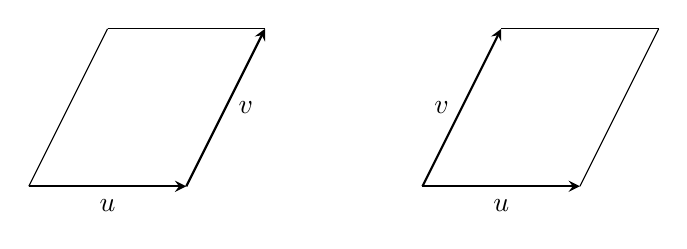
\begin{tikzpicture}[>=stealth]
    \draw[->, thick] (0,0) -- node[below=1pt] {$u$} (2,0);
    \draw (1,2) -- (3,2);
    \draw (0,0) -- (1,2);
    \draw[->, thick] (2,0) -- node[right=1pt] {$v$}(3,2);
    \draw[->, thick] (5,0) -- node[below=1pt] {$u$} (7,0);
    \draw (6,2) -- (8,2);
    \draw[->, thick] (5,0) -- node[left=1pt]{$v$} (6,2);
    \draw (7,0) -- (8,2);
    \end{tikzpicture}
    \caption{Sketch of a bivector $u \wedge v$ formed by sweeping $v$ along $u$ in contrast to the bivector $v \wedge u = - u \wedge v$, which is obtained by sweeping $u$ along $v$.}
    \label{fig:bivectors}
\end{figure}
We can represent a bivector $\omega \in \bigwedge^2 \R^3$ as a small parallelogram which suggests that we can think of it as some product of the two vectors along its sides, see figure \ref{fig:bivectors}. This is realized by the \emph{exterior product}, also called \emph{wedge product}, $u \wedge v$ of two vectors $u$ and $v$. The product $u \wedge v$ then represents the bivector obtained by sweeping $v$ along $u$. This operation yields a direct link between $\R^3$ and the vector space $\bigwedge^2 \R^3$ of bivectors, a basis of which is given by
\begin{equation}
 \{\hat{e}_1 \wedge \hat{e}_2, \hat{e}_1 \wedge \hat{e}_3, \hat{e}_2 \wedge \hat{e}_3\},
\end{equation}
if $\{\hat{e}_1, \hat{e}_2, \hat{e}_3\}$ is a basis of $\R^3$. In fact, the standard scalar product on $\R^3$ extends to a scalar product on $\bigwedge^2 \R^3$ by
\begin{equation}
( u_1 \wedge u_2 , v_1 \wedge v_2 ) = \det \left (\begin{array}{cc}
u_1 \cdot v_1 & u_1 \cdot v_2 \\ 
u_2 \cdot v_1 & u_2 \cdot v_2
\end{array}  \right).
\end{equation}
In particular, $( u \wedge v, u \wedge v ) = |u|^2 |v|^2 \sin^2\psi$, where $\psi$ is the angle between the vectors $u$ and $v$. Eventually, the norm of a bivector $\omega = \omega_{12} \hat{e}_1 \wedge \hat{e}_2 + \omega_{13} \hat{e}_1 \wedge \hat{e}_3 + \omega_{23} \hat{e}_2 \wedge \hat{e}_3$ is given by
\begin{equation}
|\omega| = \sqrt{\omega_{12}^2 + \omega_{13}^2 + \omega_{23}^2}.
\end{equation}
These definitions then extend naturally to all higher dimensions. In particular, we note that if $\{e_1, e_2, e_3, e_4\}$ again denotes the canonical basis of $\R^4$, a basis of the space $\bigwedge^2 \R^4$ is given by
\begin{equation}
\{e_{12}, e_{13}, e_{14}, e_{23}, e_{24}, e_{34}\},
\end{equation}
where we write $e_{ij} := e_i \wedge e_j$ to simplify notation.

To finish this section, we will point out some properties of the space $\bigwedge^2 \R^4$ and how it differs from $\bigwedge^2 \R^3$, which at a later point will illustrate why the optimal control curves for $\textsc{SPr3}$ and \textsc{SPr4} in general do not have the same structure.

As a matter of fact, one peculiarity of the bivectors in $\R^3$ is that they are isomorphic to the space $\R^3$ itself. This is realized by the so-called \emph{Hodge dual operator} $\star$, c.f. \cite{Lounesto2006} p. 38, which is defined in a way such that for any two vectors $u,v \in \R^3$ one has
\begin{equation}
\label{eq: hodge star}
u \wedge v = \star(u \times v),
\end{equation}
where $\times$ denotes the usual cross product. This entails two things: First, every bivector in $\R^3$ is \emph{simple}; that is, it can be written as the wegde product of two vectors. Second, every bivector in $\R^3$ defines one unique plane in $\R^3$. It is due to this underlying geometrical fact that the optimal control curves of \textsc{SPr3} are planar.

In contrast, in $\R^4$, the geometry of its bivectors proves to be more involved. As $\dim \bigwedge^2 \R^4 = 6$, it is clear that the bivectors in $\R^4$ are not isomorphic to $\R^4$ itself. In particular, in $\R^4$ not all bivectors are simple. Indeed, the bivector $e_1 \wedge e_2 + e_3 \wedge e_4 \in \bigwedge^2 \R^4$ cannot be written as an exterior product of just two vectors in $\R^4$. Nevertheless, any bivector in $\R^4$ can be written as the sum of two orthogonal simple bivectors \cite{Lounesto2006}. Moreover, we have the following criterion to determine whether a bivector is simple:


\begin{lemma}
\label{lem:simple bivector}
A bivector $\omega \in \bigwedge^2 \R^4$ is simple if and only if $\omega \wedge \omega = 0$.
\end{lemma}

\begin{proof}
If $\omega \in \bigwedge^2 \R^4$ is a simple bivector, i.e. if there are vectors $u,v \in \R^4$ such that $\omega = u \wedge v$, then it is clear from the anticommutativity and associativity of the wedge product that
\begin{equation}
\omega \wedge \omega = (u \wedge v) \wedge (u \wedge v) = - u \wedge u \wedge v \wedge v = 0.
\end{equation}
The inverse requires a rather lengthy proof by induction, see the lecture notes on projective geometry by Nigel Hitchin, chapter 3, p.48 \cite{Hitchin2003}.
\end{proof}

In what follows, we will find that the net displacement actually identifies with a bivector of $\R^4$. The solution to the optimization problem in \cite{Alouges2017} then suggests that we should be able to find a similar solution for our optimization problem, at least in the case where the net displacement is a simple bivector. The preceding lemma then serves us to identify certain subspaces of $\bigwedge^2 \R^4$ consisting only of simple bivectors. The structure of $\bigwedge^2 \R^4$ will nonetheless be crucial for the solution in the general case as well. The fact that every bivector represents in some sense two planes in $\R^4$ will indeed be the reason for the introduction of a second Fourier mode in the optimal strokes.

\subsection{G-Orthogonalization}
We begin by rewriting the energy functional (\ref{eq: linearized energy functional}) and the constraint (\ref{eq: constraint}) in terms of the orthonormal basis of eigenvectors $(\tau_i)_{i \in \N_4}$ of the matrix $G$. The change of variable $\eta(t) := U^T \xi(t) \in H_{\sharp}^{1}(J, \R^4)$, allows us to write
\begin{equation}
\label{eq: G-orth energy functional}
\mathcal{G}_{U}(\eta) = \int_{J} \Lambda_{\mathfrak{g}} \dot{\eta}(t) \cdot \dot{\eta}(t) \dd t,
\end{equation}
with $\mathcal{G}_{U}(\eta) := \mathcal{G}(\xi) = \mathcal{G}(U \eta)$. For the constraint, we note that
\begin{equation}
\det(\xi |\dot{\xi} | \tau_i | \tau_j) =  \det U \det (\eta | \dot{\eta} | e_i | e_j) = \det(\dot{\eta} | \eta | e_i |e_j),
\end{equation}
since $\det U = -1$. Eventually, we can express the determinants more elegantly in terms of exterior products. In fact, by direct calculation one obtains $\det(\dot{\eta} | \eta | e_k |e_4) = (\dot{\eta} \wedge \eta, e_{k + 1} \wedge e_{k+2})$ and $\det(\dot{\eta} |\eta | e_{k + 1} |e_{k + 2}) = (\dot{\eta} \wedge \eta, e_k \wedge e_4)$, for $k \in \N_3$ taken mod 3. Then, the isomorphism sending the standard basis $\{f_i\}_{i \in \N_6}$ of $\R^6$ onto the ordered basis 
\begin{equation}
\label{eq: basis of bivectors}
(e_{14}, e_{24}, e_{34}, e_{23}, e_{31}, e_{12})
\end{equation}
of $\bigwedge^2 \R^4$, where we write $e_{ij} := e_i \wedge e_j$, allows us to rewrite (\ref{eq: constraint}) as
\begin{equation}
\label{eq: G-orth constraint}
\Lambda_{\mathfrak{h}}^{-1} \delta p = \int_{J} \dot{\eta}(t) \wedge\eta(t) \dd t,
\end{equation}
with $\Lambda_{\mathfrak{h}} := \diag(\mathfrak{h}_{c}, \mathfrak{h}_{c}, \mathfrak{h}_{c}, \mathfrak{h}_{\theta}, \mathfrak{h}_{\theta}, \mathfrak{h}_{\theta})$.

\subsection{Fourier transformation of the minimization problem}
We denote by $\ell^2(\R^4)$ the space of sequences $\mathbf{u} := (u_n)_{n \in \N}$ in $\R^4$ such that the norm
\begin{equation}
	||\mathbf{u}||_{\ell^2(\R^4)} := \sqrt{ \sum_{n \in \N} |u_n|^2 }
\end{equation}
is finite. Consequently, we denote by $\dot{\ell}^2(\R^4)$ the Hilbert space of sequences $\mathbf{u} = (u_n)_{n \in \N} \in \ell^2(\R^4)$ such that $(n u_n)_{n \in \N} \in \ell^2(\R^4)$. As the elements in $H_{\sharp}^{1}(J, \R^4)$ are $2\pi$-periodic, we can express $\eta$ in terms of its Fourier series as
\begin{equation}
\eta(t) := \sum_{n \in \N} \cos(nt) a_n + \sin(n t) b_n,
\end{equation}
with $(a_n, b_n)_{n \in \N} \in \dot{\ell}^2(\R^4) \times \dot{\ell}^2(\R^4)$. Substitution of the Fourier series of $\dot{\eta}$ into the energy functional (\ref{eq: G-orth energy functional}) yields due to Parseval's equality
\begin{align}
\mathcal{G}_{U} (\eta) := \int_{J} \Lambda_{\mathfrak{g}} \dot{\eta}(t) \cdot \dot{\eta} dt &= \pi \sum_{n  \in \N} n^2(\Lambda_{\mathfrak{g}} a_n \cdot a_n + \Lambda_{\mathfrak{g}} b_n \cdot b_n) \\  &=
\frac{1}{2} ||\mathbf{u}||_{\ell^2(\R^4)}^2 + \frac{1}{2} ||\mathbf{v}||_{\ell^2(\R^4)}^2,
\end{align}
where we have set
\begin{align}
\label{eq:relation Fourier coeffs of eta}
	\mathbf{u} := (u_n)_{n \in \N} := \sqrt{2 \pi \Lambda_{\mathfrak{g}}}(n a_n)_{n \in \N} \text{ and } \mathbf{v} := (v_n)_{n \in \N} := \sqrt{2 \pi \Lambda_{\mathfrak{g}}} (n b_n)_{n \in \N}.
\end{align}
Clearly, we have $(\mathbf{u}, \mathbf{v}) \in \ell^2(\R^4) \times \ell^2(\R^4)$. As a result of the $L_{\sharp}^2(J, \R^4)$-orthogonality of the Fourier trigonometric system, we can express the constraint (\ref{eq: G-orth constraint}) in terms of Fourier coefficients as $2 \pi \sum_{n \in \N} \tfrac{1}{n} (nb_n) \wedge (n a_n) = \Lambda_{\mathfrak{h}}^{-1} \delta p$. Returning to our old notation for a moment, we note that for any $n \in \N$, we have
\begin{equation}
2 \pi n^2 \det(b_n | a_n | e_i | e_j) = \frac{\sqrt{\mathfrak{g}_i \mathfrak{g}_j}}{\sqrt{\det \Lambda_{\mathfrak{g}}}} \det(v_n | u_n |e_i | e_j),
\end{equation}
and hence by setting $\tilde{\Lambda}_{\mathfrak{g}} := \diag(\mathfrak{g}_c, \mathfrak{g}_c, \mathfrak{g}_c, \sqrt{\mathfrak{g}_c \mathfrak{g}_{\theta}}, \sqrt{\mathfrak{g}_c \mathfrak{g}_{\theta}}, \sqrt{\mathfrak{g}_c  \mathfrak{g}_{\theta}})$, with $\mathfrak{g}_1 :=\mathfrak{g}_2 := \mathfrak{g}_3 := \mathfrak{g}_c$ and $\mathfrak{g}_4 := \mathfrak{g}_\theta$, we eventually find
\begin{equation}
\label{eq:relation between net displacement and Fourier modes}
\sqrt{\det \Lambda_{\mathfrak{g}}} (\Lambda_{\mathfrak{h}} \tilde{\Lambda}_{\mathfrak{g}})^{-1} \delta p = \sum_{n \in \N} \frac{v_n  \wedge u_n}{n}.
\end{equation}
We thus have proved the following

\begin{proposition}
\label{prop: l2-minimization}
The $\strokes$ minimization of the functional $\mathcal{G}_U$ given by (\ref{eq: G-orth energy functional}) under the constraint (\ref{eq: G-orth constraint}) is equivalent to the minimization of the functional
\begin{equation}
\label{eq:l2-energy}
	\mathcal{F}(\mathbf{u}, \mathbf{v}) := \frac{1}{2} ||\mathbf{u} ||^2_{\ell^2(\R^4)} + \frac{1}{2} ||\mathbf{v}||^2_{\ell^2(\R^4)},
\end{equation}
defined in the product Hilbert space $\ell^2(\R^4) \times \ell^2(\R^4)$ and subject to the constraint
\begin{equation}
\label{eq:l2-constraint}
\sum_{n \in \N} \frac{1}{n} v_n \wedge u_n = \omega \text{ with } \omega := \sqrt{\det \Lambda_{\mathfrak{g}}}(\Lambda_{\mathfrak{h}} \tilde{\Lambda}_{\mathfrak{g}})^{-1} \delta p,
\end{equation}
where $\delta p \in \R^3 \times \so(3)$ is a prescribed net displacement of position and orientation.
\end{proposition}

We observe that we are in a very similar situation as in \cite{Alouges2017} with the fundamental difference however that this time the constraint is a bivector. Nevertheless, it is natural to try to generalize the approach in \cite{Alouges2017}, which in fact is true at least in the case of $\omega$ being simple. In particular, note that due to $\omega$ being related to $\delta p$ by a diagonal matrix, $\omega$ is simple if and only if $\delta p$ is simple.

\subsection[The simple case]{The simple case}
With the remarks from section \ref{sec:bivectors}, we are able to solve the constrained minimization problem of Proposition \ref{prop: l2-minimization} in a similar manner to \cite{Alouges2017} whenever the net displacement is a simple bivector. In fact, we retrieve essentially the same result, i.e. that the optimal control curves are ellipses in a certain plane defined by the net displacement. Let us prove

\begin{proposition}
\label{prop:simple reduction}
If $\omega$ is a simple bivector, then for any $(\mathbf{u}, \mathbf{v}) \in \ell^2(\R^4) \times \ell^2(\R^4)$ such that the constraint (\ref{eq:l2-constraint}) holds, there exist two vectors $u,v \in \R^4$ such that for the sequences $\mathbf{u}_{\star} := \mathbf{e}_1 u$ and $\mathbf{v}_\star := \mathbf{e}_1 v \in \ell^2(\R^4)$ one has 
\begin{equation}
\mathcal{F}(\mathbf{u_{\star}}, \mathbf{v_{\star}}) = \mathcal{F}(\mathbf{u}, \mathbf{v}) \text{ and } v \wedge u = \omega.
\end{equation}
\end{proposition}

\begin{proof}
If $\omega = 0$, then the proof is trivial. Thus, let us denote by $\hat{\omega}$ the unit bivector associated to $\omega$. For a couple $(\mathbf{u}, \mathbf{v}) \in \ell^2(\R^4) \times \ell^2(\R^4)$, we then choose $u,v \in \R^4$ such that the following relations hold:
\begin{eqnarray}
\label{eq:reduction int1}
	|u| = ||\mathbf{u} ||_{\ell^2(\R^4)}, &  |v| = ||\mathbf{v} ||_{\ell^2(\R^4)} , & \frac{v \wedge u}{|v \wedge u|} = \hat{\omega}.
\end{eqnarray}
The latter is possible since $\hat{\omega}$ is a simple bivector by hypothesis. Hence, there exist $x, y \in \R^4$ such that $\omega = x \wedge y$. Then we have for all $u, v \in \Span\{x,y\}$ such that $v \wedge u \neq 0$ that $v \wedge u/|v \wedge u| = \hat{\omega}$, up to permutation to account for the sign. Furthermore, we have $v \wedge u = ||\mathbf{u}||_{\ell^2(\R^4)} ||\mathbf{v}||_{\ell^2(\R^4)} (\sin\psi)\hat{\omega}$, where $\psi$ is the angle between $u$ and $v$. Therefore, the equality $v \wedge u = \omega$ can be satisfied by choosing the angle $\psi \in (0, \pi)$ such that
\begin{equation}
 \sin \psi = \frac{|\omega|}{||\mathbf{u}||_{\ell^2(\R^4)} ||\mathbf{v} ||_{\ell^2(\R^4)}}.
 \end{equation}
This is possible under the condition that the right hand side  of the previous equation is not greater than one. In fact, we have using the Cauchy-Schwarz inequality
\begin{equation}
|\omega| \leq \sum_{n \in \N} \frac{1}{n} |v_n \wedge u_n| \leq \sum_{n \in \N} |v_n| |u_n| \leq ||\mathbf{u} ||_{\ell^2(\R^4)} ||\mathbf{v} ||_{\ell^2(\R^4)}.
\end{equation}
Finally, from (\ref{eq:reduction int1}) we obtain
\begin{equation}
\mathcal{F}(\mathbf{u_\star}, \mathbf{v_{\star}}) = \frac{1}{2} |u|^2 + \frac{1}{2} |v|^2 = \frac{1}{2} ||\mathbf{u}||_{\ell^2(\R^4)}^2 + \frac{1}{2} ||\textbf{v}||_{\ell^2(\R^4)}^2,
\end{equation}
which concludes the proof.
\end{proof}

We immediately have

\begin{corollary}
\label{cor:simple reduction}
If $\omega$ is a simple bivector, the minimization problem for $\mathcal{F}$ in $\ell^2(\R^4) \times \ell^2(\R^4)$, under the constraint (\ref{eq:l2-constraint}), is equivalent to the minimization in $\R^4 \times \R^4$ of the function
\begin{equation}
\label{eq:finite dim energy}
 	f(u,v) := \frac{1}{2}|u|^2 + \frac{1}{2} |v|^2,
 \end{equation} 
 under the constraint
 \begin{equation}
 \label{eq:finite dim constraint}
 v \wedge u = \omega.
 \end{equation}
\end{corollary}

\begin{proof}
It suffices to observe that if $\mathcal{V}_{\omega}$ denotes the subset of $\ell^2(\R^4) \times \ell^2(\R^4)$ satisfying the constraint (\ref{eq:l2-constraint}) and by $V_{\omega}$ the subset of $(u, v)  \in \R^4 \times \R^4$ such that $v \wedge u = \omega$, then Proposition \ref{prop:simple reduction} yields
\begin{equation}
\min_{(\mathbf{u}, \mathbf{v}) \in \mathcal{V}_{\omega}}\mathcal{F}(\mathbf{u}, \mathbf{v}) = \min_{(u, v) \in V_\omega} \mathcal{F}(\mathbf{e}_1 u, \mathbf{e}_1 v) = \min_{(u,v) \in V_{\omega}} f(u,v).
\end{equation}
\end{proof}

Let us now prove the following


\begin{proposition}
\label{prop:finite dim minimization}
Any couple of vectors $(u_{\star}, v_{\star}) \in \R^4 \times \R^4$ minimizing the function $f$ given in (\ref{eq:finite dim energy}) and subject to the constraint (\ref{eq:finite dim constraint}) with $\omega = v \wedge u$ a simple bivector, is characterized by the following conditions:
\begin{eqnarray}
\label{eq:finite dim minimization conditions}
|u_{\star}|^2 = |v_{\star}|^2 = |\omega|, & 
u_{\star} \cdot v_{\star} = 0.
\end{eqnarray}
Therefore, any two vectors $\sigma, \mu \in \Span\{u, v\}$ such that $|\sigma|^2 = |\mu|^2 =|\omega|$ and $\sigma \cdot \mu = 0$, the couple $(\sigma, \mu) \in \R^4 \times \R^4$, up to permutation, is a (global) constrained minimizer for $f$.
\end{proposition}

\begin{remark}
To construct such a couple, it suffices to scale $v$ to get $v_\star$ and then find $u_\star$ by Gram-Schmidt orthogonalization and rescaling.
\end{remark}

\begin{proof}
Note that to find the minimizers of the problem (\ref{eq:finite dim energy}) - (\ref{eq:finite dim constraint}), the constraint $u \wedge v = \omega$ implies the existence of a $\psi \in (0, \pi)$ such that $|u||v| \sin \psi= |\omega|$. Hence, the constrained minimization for $f$ is equivalent to the unconstrained minimization of the function $\hat{f}: \R^4 \times (0, \pi) \to \R$ defined by
\begin{equation}
(u, \psi) \mapsto \frac{1}{2} |u|^2 + \frac{1}{2} \frac{|\omega|^2}{|u|^2 \sin^2\psi},
\end{equation}
whose stationary points satisfy $\psi_{\star} = \frac{\pi}{2}$ and $|u_{\star}|^2 = |\omega|$. This shows the necessity of the conditions stated in (\ref{eq:finite dim minimization conditions}). To show sufficiency of the condition, one observes that for any such points one has $\hat{f}(u_{\star}, \psi_{\star}) = |\omega|$. Indeed, for any $(u, \psi)  \in \R^4 \times (0, \pi)$ we have
\begin{equation}
\hat{f}(u, \psi) \geq \frac{1}{2} \frac{|u|^4 + |\omega|^2}{|u|^2} = |\omega| + \frac{1}{2}\frac{(|\omega| - |u|^2)^2}{|u|^2} \geq |\omega| = \hat{f}(u_{\star}, \psi_{\star}).
\end{equation}
A straightforward calculation shows then that for such $\sigma$ and $\mu$, one has $\sigma \wedge \mu \mid \mid \hat{\omega}$ since they are in the plane spanned by the vectors $u$ and $v$. By construction, one has $|\sigma \wedge \mu| = |\sigma| |\mu| = |\omega|$. In the case of $\sigma \wedge \mu = - \omega$, one just permutes the two vectors.
\end{proof}

Combining all the arguments above, we have our first optimality result:

\begin{theorem}
\label{thm:optimal control curves in the simple case}
Let $\delta p \in \R^3 \times \so(3) \simeq \bigwedge^2 \R^4$ be a prescribed net displacement. Moreover, assume that $\delta p$ identifies with a simple bivector. Then, any minimizer $\xi \in \strokes$ of the energy functional (\ref{eq: linearized energy functional}) subject to the constraint (\ref{eq: constraint}) is of the form
\begin{equation}
\xi(t) := (\cos t) a + (\sin t) b,
\end{equation}
i.e. an ellipse of $\R^4$ centered at the origin and contained in the plane spanned by the vectors $a$ and $b$. The vectors $a,b \in \R^4$ are obtained as follows:
\begin{enumerate}
\item We compute the vector $\omega$ via the relation
\begin{equation}
\omega := \diag \left (\frac{\sqrt{\mathfrak{g}_c \mathfrak{g}_{\theta}}}{\mathfrak{h}_c}, \frac{\sqrt{\mathfrak{g}_c \mathfrak{g}_{\theta}}}{\mathfrak{h}_c}, \frac{\sqrt{\mathfrak{g}_c \mathfrak{g}_{\theta}}}{\mathfrak{h}_c}, \frac{\mathfrak{g}_c}{\mathfrak{g}_\theta}, \frac{\mathfrak{g}_c}{\mathfrak{g}_\theta}, \frac{\mathfrak{g}_c}{\mathfrak{g}_\theta} \right ) \delta p \simeq v \wedge u,
\end{equation}
where we may assume that $u \cdot v = 0$ and $|u| = |v| = \sqrt{|\omega|}$.

\item We calculate the vectors $a$ and $b$ via the relations
\begin{equation}
\label{eq:global minimizer form}
\begin{aligned}
a := \frac{U \Lambda_{\mathfrak{g}}^{-1/2}}{\sqrt{2 \pi}} u,&& b := \frac{U \Lambda_{\mathfrak{g}}^{-1/2}}{\sqrt{2 \pi}} v.
\end{aligned}
\end{equation}
\end{enumerate}

In addition, the minimal value of the energy functional is $|\omega|$, and the vectors $a$ and $b$ are $\mathfrak{g}$-orthogonal, i.e. with respect to the inner product defined for every $x,y \in \R^4$ by $(x, y)_{\mathfrak{g}} := 2 \pi \Lambda_{\mathfrak{g}} x \cdot y$, and have the same $\mathfrak{g}$-norm $|a|_{\mathfrak{g}}^2 = |b|_{\mathfrak{g}}^2 = |\omega|$. 
\end{theorem}


\begin{proof}
From Proposition \ref{prop:finite dim minimization}, Corollary \ref{cor:simple reduction} and then Proposition \ref{prop: l2-minimization}, we get that any $u, v \in \R^4$ satisfying the relations
\begin{eqnarray}
v \wedge u = \omega,  &  u \cdot v = 0, &  |u|^2 = |v|^2 =  |\omega|,
\end{eqnarray}
 with $\omega := \sqrt{\det \Lambda_{\mathfrak{g}}} (\Lambda_{\mathfrak{h}} \tilde{\Lambda}_{\mathfrak{g}})^{-1} \delta p$, is associated to a (global) constrained minimizer for $\mathcal{G}_{U}$, via the curve $\eta(t) := (\cos t) \tilde{a} + (\sin t) \tilde{b}$, where the Fourier coefficients $\tilde{a}, \tilde{b} \in \R^4$ are related to $\omega$ (c.f. \ref{eq:relation Fourier coeffs of eta}) by $(\sqrt{2 \pi \Lambda_{\mathfrak{g}}}) \tilde{a} = u$ and $(\sqrt{2 \pi \Lambda_{\mathfrak{g}}}) \tilde{b} = v$. The minimum value of the energy is then $\mathcal{G}_{U}(\eta) = |\omega|$.

Finally, in the $\mathfrak{g}$-orthogonal reference frame, the inner product is defined by $(x, y)_{\mathfrak{g}} := 2 \pi \Lambda_{\mathfrak{g}}x \cdot y$ for $x,y \in \R^4$. Let us denote by $|\cdot|_{\mathfrak{g}}$ the associated norm. Then we have the following relations:
\begin{align}
|\tilde{a}|_{\mathfrak{g}}^2 = |\tilde{b}|_{\mathfrak{g}}^{2} = |\omega| \;  \text{ and } \; (\tilde{a}, \tilde{b})_{\mathfrak{g}} = 0.
\end{align}
Applying the orthogonal map $U$ to $\tilde{a}$ and $\tilde{b}$ finishes the proof.
\end{proof}

\subsubsection{Examples of simple net displacements}
In light of Theorem \ref{thm:optimal control curves in the simple case} presented above, one might ask whether there are concrete cases in which the net displacement happens to be a simple bivector. It turns out that there is convenient correspondence for engineering purposes between certain subspaces of $\bigwedge^2 \R^4$ consisting only of simple bivectors and certain net displacements. First, note that purely spatial net displacements are always simple since one can always factor out $e_4$ from all three corresponding basis vectors, cf. (\ref{eq: basis of bivectors}). Moreover, observe that the condition in Lemma \ref{lem:simple bivector} is in particular satisfied if all coefficients corresponding to a certain index are zero, e.g. $\omega_{i4} = 0$ for $i \in \N_3$. This yields four subspaces $D_{ijk} \subset \bigwedge^2 \R^4$ consisting only of simple bivectors. Then, by inspection of the basis of $\bigwedge^2 \R^4$, we find the correspondences displayed in table \ref{tab:simple net displacements}.
\begin{table}[h]
    \centering
        \begin{tabular}{cl}
        \toprule 
        \textit{Subspace} & \textit{Corresponding net displacements} \\ 
        \midrule 
        $D_{123}$ & rotations around all three axes  $\hat{e}_1, \hat{e}_2$, and $\hat{e}_3$ \\ 
        % \hline 
        $D_{124}$ & translation in the $\hat{e}_1\hat{e}_2$-plane, rotation around the $\hat{e}_3$-axis \\ 
        % \hline 
        $D_{134}$ & translation in the $\hat{e}_1\hat{e}_3$-plane, rotation around the $\hat{e}_2$-axis  \\ 
        % \hline 
        $D_{234}$ & translation in the $\hat{e}_2\hat{e}_3$-plane, rotation around the $\hat{e}_1$-axis  \\ 
        \bottomrule 
        \end{tabular} 
    \caption{Correspondences between subspaces of $\bigwedge^2 \R^4$ consisting of simple bivectors and net displacements in $\R^3\times \SO(3)$.}
    \label{tab:simple net displacements}
\end{table}

By comparison, the non-simple bivector $e_{12} + e_{34}$ corresponds to the net displacement $e_3 + L_3$, i.e. a screw motion. This kind of movement requires a solution to the general problem, which we treat in the following section.


\subsection{The general case}

Let us now address the case of a general net displacement, i.e. $\delta p \in \R^6 \simeq \bigwedge^2 \R^4$ which identifies to a non-simple bivector. Recall that every simple bivector represents a plane in $\R^4$, while we can always express an arbitrary bivector in $\bigwedge^2 \R^4$ as the sum of two orthogonal simple bivectors. Therefore, the observations from section \ref{sec:bivectors} suggest that the optimal curve in the general case consists of two ellipses in two planes. We will indeed be able to prove this result. However, we first have to return to variational calculus to do so.


\subsubsection{The optimization problem in the variational setting}
More precisely, we will establish the structure of the optimal control curves using the Euler-Lagrange equation associated with the optimization problem. To that end, let us recast the optimization problem in its original form:
\begin{align}
\label{eq:original_optimization_problem}
\begin{cases}
 \text{Find } \min_{\xi \in \dot{H}^1_{\sharp}} \int_{J} G \dot{\xi}(t) \cdot \dot{\xi}(t) \dd t\\
 \text{under the constraints }\\
 \int_{J} M_i \dot{\xi}(t) \cdot \xi(t) \dd t = \delta p_i,\, i \in \N_6.
 \end{cases}
\end{align}
Accordingly, we are in the setting of a variational problem with six isoperimetric constraints. For $i \in \N_6$, denote by $K_i: \strokes \times L^2_\sharp(J, \R^4) \times J \to \R$ the map
\begin{align}
	K_i(\xi, \eta, t) := M_i \eta(t) \cdot \xi(t).
\end{align}
Furthermore, denote by $\mathcal{K}_i : \strokes \to \R$ the functional
\begin{align}
	\mathcal{K}_i(\xi) := \int_{J} K_i(\xi, \dot{\xi}, t) \dd t.
\end{align}
Then, the six isoperimetric constraints read $\mathcal{K}_i(\xi) = \delta p_i$ for $i \in \N_6$. Now, let us denote by $\delta \mathcal{G}$ and $\delta \mathcal{K}_i$ the first variations of $\mathcal{G}$ and the $\mathcal{K}_i$, respectively. Then a slight adaptation of Proposition 2.1.3. in \cite{Kielhoefer2018} shows that $\xi \in \strokes$ is a minimizer of (\ref{eq:original_optimization_problem}) and if $\xi$ is not critical for the constraints, i.e. $\delta \mathcal{K}_1(\xi), \dotsc, \delta \mathcal{K}_6(\xi)$ are linearly independent, then $\xi$ satisfies the Euler-Lagrange equation:

\begin{align}
\label{eq:euler_lagrange}
\frac{\dd}{\dd t} \frac{\partial}{\partial \dot{\xi}} \left ( G \dot{\xi}(t) \cdot \dot{\xi}(t) + \sum_{i \in \N_6} \mu_i K_i(\xi, \dot{\xi}, t)\right ) = \frac{\partial}{\partial \xi} \left ( G \dot{\xi}(t) \cdot \dot{\xi}(t) + \sum_{i \in \N_6} \mu_i K_i(\xi, \dot{\xi}, t)\right ),
\end{align}
for some $\mu \in \R^6$. To make use use of equation (\ref{eq:euler_lagrange}), let us prove the following result.

\begin{proposition}
\label{prop:linearly_independent_constraints}
Let $\delta p \in \R^6 \simeq \bigwedge^2 \R^4$ be non-simple and $\xi \in \strokes$ a minimizer of (\ref{eq:original_optimization_problem}). Then the functionals $\delta \mathcal{K}_1(\xi), \dotsc, \delta \mathcal{K}_6(\xi)$ are linearly independent.
\end{proposition}

\begin{proof}
Let $\lambda_1, \dotsc, \lambda_6 \in \R$ be such that $\sum_{i \in \N_6} \lambda_i \delta \mathcal{K}_i(\xi) $ is the zero functional in the dual space of $\strokes$. Note that by the periodicity of $\xi$ and integration by parts, we have for any $h \in \strokes$ that
\begin{align}
	\delta \mathcal{K}_i(\xi) h =  2 \int_J M_i \dot{\xi}(t) \cdot h(t) \dd t.
\end{align}
Setting $\Omega(\lambda) := \sum_{i \in \N_6} \lambda_i M_i$ for $\lambda \in \R^6$, we find that the functional $h \in \strokes \mapsto \int_J \Omega(\lambda) \dot{\xi}(t) \cdot h(t) \dd t$ is the zero functional. For the time being, let us choose $h = \Omega(\lambda) \dot{\xi}$, but note that $h$ is not necessarily in $\strokes$. Then we have
\begin{align}
\label{eq:zero_functional}
	0 = \int_J \Omega(\lambda) \dot{\xi}(t) \cdot h(t) \dd t = ||h||_{L^2}^{2},
\end{align}
i.e. $h \equiv 0$ almost everywhere. This can only happen in the two cases $\xi(t) \in \ker \Omega(\lambda)$ for all $t \in J$ or $\lambda_1 = \dotsm = \lambda_6 = 0$, in the latter of which we are done. So, let us suppose that we are in the former case. Note that the matrix $\Omega(\lambda)$ is skew symmetric. Hence, we find an orthogonal transformation $S$ such that $\Omega(\lambda) = S \Sigma(\lambda) S^T$ with

\begin{align}
\Sigma(\lambda) = \diag \left (\left( \begin{array}{cc}
0 & \nu_+(\lambda) \\ 
- \nu_+ (\lambda) & 0
\end{array} \right ) , \left ( \begin{array}{cc}
0 & \nu_{-}(\lambda) \\ 
- \nu_{-}(\lambda) & 0
\end{array} \right ) \right ).
\end{align}
Denoting by $P$ and $Q$ the projections $\R^6 \to \R^3$ on the first respectively the last three coordinates, the scalars $\nu_{\pm}$ are given by
\begin{align}
	\nu_{\pm} = 2 \sqrt{3} \sqrt{A \pm \sqrt{A^2 - K}},
\end{align}
with $A := \alpha^2 |P \lambda|^2 + \delta^2 |Q \lambda|^2$ and $K := 4 \alpha^2 \delta^2 |P\lambda \cdot Q \lambda|^2$. Hence, only $\nu_-$ can vanish, which implies that $\ker \Omega(\lambda)$ is at most of dimension two. However, this is excluded by the Lemma below, as $\delta p$ is assumed to be non-simple. Thus, we have $||h||_{L^2} > 0$. Now, approximation of $\dot{\xi}$ by smooth functions shows that $h \in \strokes \mapsto \int_J \Omega(\lambda) \dot{\xi}(t) \cdot h(t) \dd t$ cannot be the zero functional. Therefore, we must have $\lambda_1 = \dotsm = \lambda_6 = 0$, which finishes the proof.
\end{proof}

The following Lemma completes the proof of Proposition \ref{prop:linearly_independent_constraints}:
\begin{lemma}
	Let $\xi \in \strokes$ be a control curve. Suppose that $\xi(t) \in D$ for all $t \in J$, where $D \subset \R^4$ is a plane through the origin. Then, the net displacement due to $\xi$ is a simple bivector.
\end{lemma}

\begin{proof}
Note that if $\xi$ only takes values in the plane $D$, then the rescaled Fourier coefficients in relation (\ref{eq:l2-constraint}) must also lie in a plane $D'$ (not necessarily the same). Hence, the net displacement due to $\xi$ lies in fact in $\bigwedge^2 D'$. Thus, it must be simple since $D'$ is of dimension two and consequently $\dim \bigwedge^2 D' = 1$.
\end{proof}

\subsubsection{Structure of the solutions to the Euler-Lagrange equation}

By direct computation, one finds that after integration and utilizing the fact that $\xi$ is of average zero, the Euler-Lagrange equation (\ref{eq:euler_lagrange}) reads
\begin{equation}
\label{eq:euler_lagrange_integrated}
G \dot{\xi} - \Omega(\mu) \xi = 0,
\end{equation}
where $\Omega(\mu)$ is the skew symmetric matrix from (\ref{eq:zero_functional}). To reveal the structure of the solutions to (\ref{eq:euler_lagrange_integrated}), we need to apply two basis transformations: First, setting $\eta := G^{1/2} \xi$ yields
\begin{equation}
\dot{\eta} - \tilde{\Omega}(\mu) \eta = 0,
\end{equation}
where $\tilde{\Omega}(\mu) := \sum_{i \in \N_6} \mu_i G^{-1/2} M_i G^{-1/2}$, which is still a skew symmetric matrix. Hence, we find an orthogonal transformation $Q$ such that $\tilde{\Omega} = Q \tilde{\Sigma}(\mu) Q^T$ with
\begin{align}
	\tilde{\Sigma}(\mu) \diag \left (\left( \begin{array}{cc}
0 & \sigma_1(\mu) \\ 
- \sigma_1(\mu) & 0
\end{array} \right ) , \left ( \begin{array}{cc}
0 & \sigma_2(\mu) \\
- \sigma_2(\mu) & 0
\end{array} \right ) \right ).
\end{align}
Consequently, setting $\phi := Q \eta$, we have the equation $\dot{\phi} = \tilde{\Sigma}(\mu) \phi$, the solution of which is given by $\phi(t) = \exp \left ( \tilde{\Sigma}(\mu) t \right )\phi_0$ with $\phi_0 := QG^{1/2}\xi(0)$. By defining the vectors
\begin{align}
	\phi_{\sigma_1} &:= (\phi_{0,1}, \phi_{0,2}, 0, 0)^T,  & \psi_{\sigma_1} &:= (\phi_{0,2}, - \phi_{0,1}, 0, 0)^T,\\
	\phi_{\sigma_2} &:= (0,0,\phi_{0,3}, \phi_{0, 4})^T,  & \psi_{\sigma_2} &:= (0,0,- \phi_{0,4}, \phi_{0,3})^T,
\end{align}
and explicitly calculating $\exp(\tilde{\Sigma}(\mu)t)$, we can recast the curve $\phi$ as
\begin{eqnarray}
\phi(t) = \sum_{i \in \N_2} [\cos(\sigma_i(\mu)t) \phi_{\sigma_i} + \sin(\sigma_i(\mu)t) \psi_{\sigma_i}], & & t \in J.
\end{eqnarray}
Resubstituting the basis transformations, we find that $\xi$ must be of the form
\begin{eqnarray}
\label{eq:general_optimal_curve}
\xi(t) = \sum_{i \in \N_2} [\cos(\sigma_i(\mu)t) a_{\sigma_i} + \sin(\sigma_i(\mu)t) b_{\sigma_i}], & & t \in J.
\end{eqnarray}
Note that the vectors $\phi_{\sigma_1}, \psi_{\sigma_1}, \phi_{\sigma_2}$ and $\psi_{\sigma_2}$ are pairwise orthogonal. So, $\phi$ is in fact a rotation in two completely orthogonal planes of $\R^4$. In particular, this implies that the vectors $a_{\sigma_1}, b_{\sigma_1}, a_{\sigma_2}$ and $b_{\sigma_2}$ are orthogonal in the reference system of $G$.

\subsubsection{Existence of integer eigenvalues}
It is clear that the eigenvalues $\sigma_1(\mu)$ and $\sigma_2(\mu)$ must be integers for the curve $\xi$ in (\ref{eq:general_optimal_curve}) to be periodic. Hence, we must be able to choose $\mu \in \R^6$ such that $\sigma_1(\mu), \sigma_2(\mu) \in \N$. This question is addressed in this subsection.

First, note that we cannot have $\sigma_1(\mu) = \sigma_2(\mu)$ since then there would be only one Fourier mode and thus the relation (\ref{eq:relation between net displacement and Fourier modes}) would imply that $\delta p$ is simple. Next, one finds that the eigenvalues are given by
\begin{align}
	\sigma_{1,2}(\mu) = \frac{2 \sqrt{3}}{g_c \sqrt{g_\theta}} \sqrt{A \mp \sqrt{A^2 - K}},
\end{align}
where this time $A := \alpha^2 g_c |P \mu|^2 + \delta^2 g_{\delta} |Q \mu|^2 \geq 0$ and $K := 4 \alpha^2 \delta^2 g_c g_\theta |P\mu \cdot Q \mu|^2 \geq 0$. Clearly, we have $\sigma_2(\mu) \geq \sigma_1(\mu)$. So let us find the values for $\mu \in \R^6$ such that
\begin{eqnarray}
\label{eq:integer_condition}
	\sigma_1(\mu) = k \in \N \text{ and } \sigma_2(\mu) = lk, & & l \in \N.
\end{eqnarray}
This does not cover all possible pairs of integers. However, we will see in the next subsection that this is sufficient.

Imposing the two equations above on the eigenvalues leads to the definition of the quadratic form associated to the positive definite matrix
\begin{align}
	\Gamma := \frac{48}{g_c^2 g_\theta} \left (\begin{array}{cc}
	\alpha^2 g_c I_3 & 0 \\ 
	0 & \delta^2 g_\theta I_3
	\end{array}  \right ).
\end{align}
Indeed, one can show that the solution sets to (\ref{eq:integer_condition}) are given by $E_+^{k,l} \cup E_{-}^{k,l}$, where
\begin{align}
E_+^{k,l} := \{\mu \in \R^6 \mid \Gamma \mu \cdot \mu = \tfrac{(1 + l^2)k^2}{l^2}\} \text{ and } E_{-}^{k,l} := \{\mu \in \R^6 \mid \Gamma \mu \cdot \mu = (1 + l^2)k^2\},
\end{align}
i.e. the solutions are the union of two specific ellipsoids in $\R^6$. Note in particular, that this calculation covers the case $\sigma_1(\mu) = 1$ and $\sigma_2(\mu) = 2$. So, we have assured the existence of periodic solutions to the Euler-Lagrange equation and we will show in the following subsection that the latter choice of values for the eigenvalues is indeed optimal.

\subsubsection{Optimal control curves}
As of yet, the geometric structure of the optimal control curves is clear from (\ref{eq:general_optimal_curve}). So, let us now settle their explicit construction from a given non-simple net displacement. To that end, let us transform the Fourier modes $a_{\sigma_1}, b_{\sigma_1}, a_{\sigma_2}$ and $b_{\sigma_2}$ to the $G$-orthogonal reference by setting $\tilde{a}_{\sigma_1} := U^Ta_{\sigma_1}$ and similarly for the others. Then, substituting the curve into the energy functional $G$ yields
\begin{align}
\label{eq:optimal_energy}
	\mathcal{G}(\xi) = \pi \sigma_1(\mu)^2[\Lambda_{\mathfrak{g}}\tilde{a}_{\sigma_1} \cdot \tilde{a}_{\sigma_1} + \Lambda_\mathfrak{g} \tilde{b}_{\sigma_1} \cdot \tilde{b}_{\sigma_1}] + \pi \sigma_2(\mu)^2[\Lambda_{\mathfrak{g}} \tilde{a}_{\sigma_2} \cdot \tilde{a}_{\sigma_2} + \Lambda_{\mathfrak{g}}\tilde{b}_{\sigma_2} \cdot \tilde{b}_{\sigma_2}]\\
	=\frac{\sigma_1(\mu)}{2} [|u_{\sigma_1}|^2 + |v_{\sigma_1}|^2] + \frac{\sigma_2(\mu)}{2}[|u_{\sigma_2}|^2 + |v_{\sigma_2}|^2],
\end{align}
with 
\begin{eqnarray}
\label{eq:relation of decomposition to Fourier coeffs}
	u_{\sigma_i} := \sqrt{2 \pi \sigma_i(\mu) \Lambda_\mathfrak{g}}\tilde{a}_{\sigma_i} &\text{ and }& v_{\sigma_i} := \sqrt{2 \pi \sigma_i(\mu) \Lambda_{\mathfrak{g}}} \tilde{b}_{\sigma_i},
\end{eqnarray}
for $i \in \N_2$. In particular, it follows from relation (\ref{eq:relation between net displacement and Fourier modes}) that
\begin{equation}
	\sqrt{\det \Lambda_{\mathfrak{g}}}(\Lambda_{\mathfrak{h}} \Lambda_{\mathfrak{g}})^{-1} \delta p = v_{\sigma_1} \wedge u_{\sigma_1} + v_{\sigma_2} \wedge u_{\sigma_2}.
\end{equation}
We observe that the latter relation in the sense of (\ref{eq:relation between net displacement and Fourier modes}) is independent of the indices $\sigma_1$ and $\sigma_2$.  So, we can choose $\sigma_1(\mu) = 1$ and $ \sigma_2(\mu) = 2$ up to permutation such that $|u_{\sigma_1}|^2 + |v_{\sigma_1}|^2 \geq |u_{\sigma_2}|^2 + |v_{\sigma_2}|^2$. This choice of frequencies minimizes the energy in (\ref{eq:optimal_energy}). Recall that it has been shown in the previous section, that we can indeed find $\mu \in \R^6$, which realizes $\sigma_1(\mu) = 1$ and $\sigma_2(\mu) = 2$

Moreover, note that the vectors $u_{\sigma_1}, v_{\sigma_1}, u_{\sigma_2},$ and $v_{\sigma_2}$ are pairwise orthogonal due to the $G$-orthogonality of $a_{\sigma_1}, b_{\sigma_1}, a_{\sigma_2},$ and $b_{\sigma_2}$. Eventually, due to the bilinearity of the exterior product, we can always suppose that $|u_{\sigma_1}| = |v_{\sigma_1}|$ and $|u_{\sigma_2}| = |v_{\sigma_2}|$, which then fully minimizes the energy. One can see this by slightly adapting Proposition \ref{prop:finite dim minimization}. Conversely, note that once we are given a decomposition of $\omega  = 	\sqrt{\det \Lambda_{\mathfrak{g}}}(\Lambda_{\mathfrak{h}} \Lambda_{\mathfrak{g}})^{-1} \delta p$ into the sum of two orthogonal simple bivectors, the equations in (\ref{eq:relation between net displacement and Fourier modes}) give us a direct relation between the prescribed net displacement and the Fourier coefficients of the optimal control curve. Finally, let us summarize the above argument as follows.

\begin{theorem}
\label{thm:optimal_control_curves_general_case}
Let $\delta p \in \R^6 \simeq \bigwedge^2 \R^4$ a net displacement identifying to a non-simple bivector, then the energy minimizing curve which attains $\delta p$ is given by
\begin{eqnarray}
\xi(t) := \cos(t) a_1 + \sin(t) b_1 + \cos(2t) a_2 + \sin(2t) b_2,& t \in J,
\end{eqnarray}
where the vectors $a_1, b_1,a_2, b_2 \in \R^4$ are determined as follows:
\begin{enumerate}
\item First, we decompose the bivector $\omega := \sqrt{\det \Lambda_{\mathfrak{g}}}(\Lambda_{\mathfrak{h}} \tilde{\Lambda}_{\mathfrak{g}})^{-1} \delta p$ into the sum of two orthogonal simple bivectors, i.e.
\begin{align}
	\omega = v_1 \wedge u_1 + v_2 \wedge u_2,
\end{align}
with  all four vectors $u_1, u_2, v_1, v_2$ pairwise orthogonal and  $|u_i| = |v_i|$, for $i \in \N_2$.

\item If necessary, we permute the indices such that $|u_2|^2 + |v_2|^2 \leq |u_1|^2 + |v_1|^2$.

\item We set
	\begin{align}
		a_1 := \frac{U \Lambda_{\mathfrak{g}}^{-1/2}}{\sqrt{2 \pi}} u_1 &, & b_1 := \frac{U \Lambda_{\mathfrak{g}}^{-1/2}}{\sqrt{2 \pi}}v_1,\\
	a_2 := \frac{U \Lambda_{\mathfrak{g}}^{-1/2}}{\sqrt{4 \pi}} u_2& , & b_2 := \frac{U \Lambda_{\mathfrak{g}}^{-1/2}}{\sqrt{4 \pi}} v_2.	
	\end{align}
\end{enumerate}
Then the four vectors $a_1, b_1, a_2, b_2$ are $\mathfrak{g}$-orthogonal and the minimum value of the energy functional is $\frac{1}{2} [|u_1|^2 + |v_1|^2] +  [|u_2|^2 + |v_2|^2]$.
\end{theorem}

\begin{remark}
We point out here that in the simple case, we automatically retrieve the result from Theorem \ref{thm:optimal control curves in the simple case}.
Note also that in the simple case, the energy consumed by a energy minimizing stroke $\xi_*$ was $\mathcal{G}(\xi_*) = |\omega|$ for $\omega = \sqrt{\det \Lambda_{\mathfrak{g}}}(\Lambda_{\mathfrak{h}} \tilde{\Lambda}_{\mathfrak{g}})^{-1} \delta p$. In the general case, where $\omega = v_1 \wedge u_1 + v_2 \wedge u_2$, where the four vectors are mutually orthogonal and $|u_i| = |v_i| := l_i$ for $i \in \N_2$, we have by the Pythagorean Theorem that $|w|^2 = |l_1|^4 + |l_2|^4$. So, for a minimizer $\xi_*$ of the general problem, we find the estimate $\mathcal{G}(\xi_*) = l_1^2 + 2 l_2^2 \leq 3 |\omega|$. This allows us to frame the energy consumption by minimizing control curves in terms of the norm of the net displacement.
\end{remark}

\subsubsection{Non-uniqueness of optimal curves}
\label{subsec:non_uniqueness}
To end this section, we want to highlight a striking feature of the control system associated to the swimmer \textsc{SPr4}, namely that the optimal control curves are not necessarily unique. This follows readily from the fact that the decomposition of a bivector $\omega \in \bigwedge^2 \R^4$ into the sum of two orthogonal simple bivectors is not unique when the norms of the two summands are equal \cite{Lounesto2006}. Indeed, consider the net displacement $\delta p \in \R^3 \times \so(3) \simeq \bigwedge^2 \R^4$ such that
\begin{equation}
    \omega =  \sqrt{\det \Lambda_{\mathfrak{g}}}(\Lambda_{\mathfrak{h}} \tilde{\Lambda}_{\mathfrak{g}})^{-1} \delta p = e_1 \wedge e_2 + e_3 \wedge e_4.
\end{equation}
Clearly, the two summands on the right hand side are of equal norm. In fact, we have the second equation
\begin{equation}
\label{eq:non_unique_decomposition}
    \omega = e_1 \wedge e_2 + e_3 \wedge e_4 = \tfrac{1}{2}(e_1 + e_3) \wedge (e_2 + e_4) + \tfrac{1}{2}(e_1 - e_3)\wedge(e_2 - e_4).
\end{equation}
Hence, the construction in Theorem \ref{thm:optimal_control_curves_general_case} yields two distinct control curves which realize the same net displacement using the same (optimal) amount of energy. The different trajectories of \textsc{SPr4} due to the two distinct optimal control curves in the limit of very long arms are displayed in figure \ref{fig:non_unique_curves}, where we had to rescale $\delta p$ appropriately, for details see sections \ref{sec:laa} and \ref{sec:numerics}.
\begin{figure}[h]
    \centering
    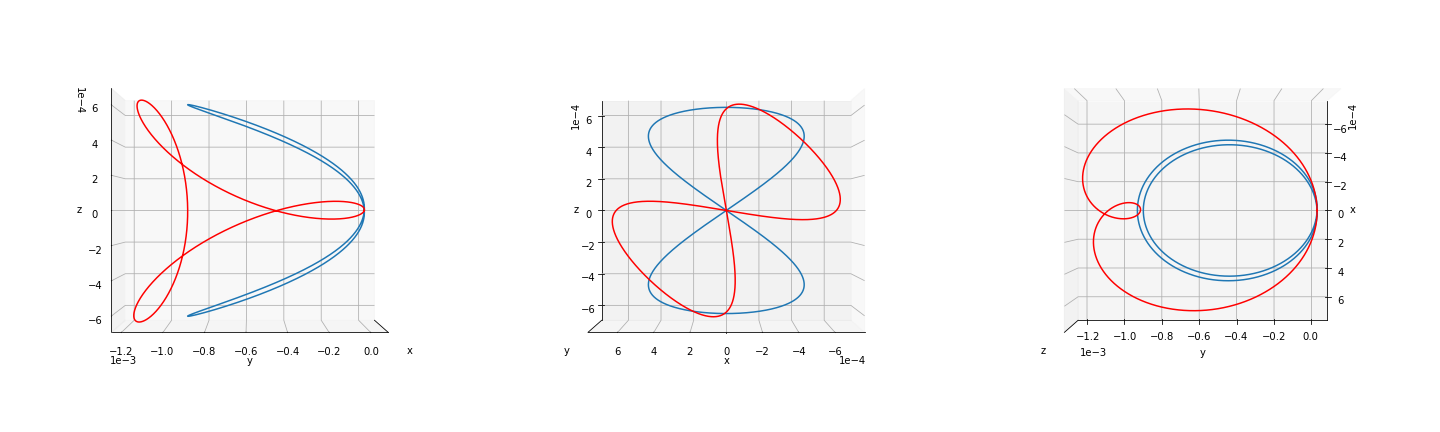
\includegraphics[width = \textwidth]{images/non_unique_curves.png}
    \caption{The tractectories of \textsc{SPr4} in the limit of very long arms due to the two distinct optimal control curves resulting from the two decompositions in (\ref{eq:non_unique_decomposition}), shown (from left to right) in frontal view, side view and top view. The red trajectory corresponds to the left decomposition, while the blue trajectory corresponds to the right one.}
    \label{fig:non_unique_curves}
\end{figure}






\printbibliography[title = Bibliography]



\end{document}